%------------------------------------------------------------
% DEFINITIONS AND HEADERS -- IGNORE THIS
%------------------------------------------------------------
\documentclass{article}
\usepackage[top=2.0cm, bottom=3cm, left=2.25cm, right=2.20cm]{geometry}
\usepackage[utf8]{inputenc}
\usepackage{algpseudocode}
% Get better typography
\usepackage[protrusion=true,expansion=true]{microtype}
% For algorithms
\usepackage[boxruled,linesnumbered,vlined,inoutnumbered]{algorithm2e}
\SetKwInOut{Parameter}{Parameters}
% For basic math, align, fonts, etc.
\usepackage{amsmath}
\usepackage{amsthm}
\usepackage{amssymb}
\usepackage{mathtools}
\usepackage[table,xcdraw]{xcolor}
\usepackage{colortbl}
\usepackage{mathrsfs}
\usepackage{rotating}
\usepackage[table,xcdraw]{xcolor}
\usepackage{colortbl}
\usepackage{tabularx}
\usepackage{float}
\usepackage{booktabs}
\usepackage{soul}
\usepackage{changepage}
\usepackage{gensymb} % For \degree
\usepackage{lscape}
% For \thead to make line breaks in tables
\usepackage{array}
\usepackage{makecell}
\renewcommand\theadalign{bc}
\renewcommand\theadfont{\bfseries}
\renewcommand\theadgape{\Gape[4pt]}
\renewcommand\cellgape{\Gape[4pt]}
\usepackage{courier} % For \texttt{foo} to put foo in Courier (for code / variables)
\usepackage{lipsum} % For dummy text
% For images
\usepackage{graphicx}
\usepackage{subcaption}
\usepackage[space]{grffile} % For spaces in image names
% For bibliography
\usepackage[round]{natbib}
% For color
\usepackage{xcolor}
\definecolor{light-grey}{rgb}{0.9,0.9,0.9}
\definecolor{dark-red}{rgb}{0.4,0.15,0.15}
\definecolor{dark-blue}{rgb}{0,0,0.7}
\definecolor{darkblue}{rgb}{0,0,.6}
\definecolor{darkred}{rgb}{.58,0,0}
\definecolor{brighterred}{rgb}{.745,0,0}
\definecolor{darkgreen}{rgb}{0,.6,0}
\definecolor{red}{rgb}{.98,0,0}
\usepackage{environ}
% Only show sections in table of contents and rename
\setcounter{tocdepth}{2}
\renewcommand{\contentsname}{Table of Contents}
% For links (e.g., clicking a reference takes you to the phy)
\usepackage{hyperref}
\hypersetup{
    colorlinks, linkcolor={dark-blue},
    citecolor={dark-blue}, urlcolor={dark-blue}
}
\newcommand{\HIGHLIGHT}[1]{\textcolor{blue}{\textbf{#1}}}
% \newcommand{\Solution}[1]{{\color{blue} \paragraph{\bf $\bigstar $ SOLUTION:} { \sf
%     #1} \bigskip}}
\newcommand{\TODO}[1]{\textcolor{blue}{\textbf{{#1}}}}
\newcommand{\POINTS}[1]{\textcolor{purple}{\textbf{{#1}}}}
\providecommand{\mathcolor}[2]{\textcolor{#1}{#2}}
% My definition of "summary boxes" (see below)
\usepackage[most]{tcolorbox}
\definecolor{boxgray}{rgb}{0.95, 0.95, 0.95}
\definecolor{boxblue}{rgb}{0.941, 0.941, 0.98}
\definecolor{boxpink}{rgb}{1.0, 0.93, 0.93}
\definecolor{boxwhite}{rgb}{1.0, 1.0, 1.0}
%\definecolor{boxgreen}{rgb}{0.91, 0.96, 0.9}
\definecolor{boxgreen}{rgb}{0.92, 0.96, 0.92}
\newtcolorbox{mybox}[1][boxwhite]{%
  enhanced,
  boxrule=0.5pt,
  colframe=black,
  colback=#1,
  sharp corners,
  width=\linewidth,
  left=1em,
  right=1em,
  top=0.5em,
  bottom=0.5em,
  boxsep=0pt,
  before skip=1em,
  after skip=0.85em,
}


\begin{document}
%-----------------
%   Homework 1
%-----------------
\newpage
\vspace*{1cm}
\begin{center}
    \begin{Large}
    {\Huge \textbf{COMPSCI 589 - Machine Learning}}\\
    \vspace{0.2cm}
    {\Huge \textbf{Final Project Report - Spring 2026}}
    \end{Large}
    \\
    \vspace{1.00cm}
        {\LARGE \textbf{Students Name:}}\\
        \vspace{0.60cm}
        {\LARGE \textbf{Jesse Chamberlain}}\\
        \vspace{0.45cm}
        {\LARGE \textbf{Mohan Kumar Paramasivan}}\\
        \vspace{0.45cm}
        {\LARGE \textbf{Monica Hernandez Lordui}}
        \vspace{0.45cm}
\end{center}
\addcontentsline{toc}{subsection}{\textbf{Final Project}}

\vspace{0.5cm}
\section*{Notes}
\vspace{0.5cm}

\begin{itemize}
    \item Code available at: \url{https://github.com/JesseChamberlain/CS589_final_group_project}
    \item \textbf{Jesse Chamberlain} - Hand-written Digits Recognition Dataset, and Rice Grains Dataset
    \item \textbf{Mohan Kumar Paramasivan} - Oxford Parkinson’s Disease Detection Dataset
    \item \textbf{Monica Hernandez Lordui} - Credit Approval Dataset
\end{itemize}
\vspace{0.8cm}
\noindent {\LARGE{\textbf{1. Evaluate the performance}}} \POINTS{}

\vspace{0.45in}
\noindent {\Large{\textbf{A.} \textbf{The Hand-Written Digits Recognition Dataset}}}
\vspace{0.5cm}
\noindent k-NN and Random Forest algorithms were also chosen for the handwritten dataset. The digits experiment stresses the algorithms far differently than the Rice experiment. With 10 classes and 64 pixel features and affixed feature scale, it provides an interesting contrast of reactions to different datasets to the same algorithms.
\vspace{0.5cm}

\noindent {\Large{\textbf{B.} \textbf{The Oxford Parkinson’s Disease Detection Dataset}}}\\

\noindent Neural Networks were selected for the Oxford Parkinson’s Disease Detection Dataset because the dataset consists of numerical biomedical voice measurements with complex underlying patterns. Neural Networks are highly effective for pattern recognition and classification tasks, especially when relationships between input features are nonlinear. The model analyzes the voice measurements of individuals, learns important speech-related patterns, and predicts whether the patient has Parkinson’s disease or not.\\

The K-Nearest Neighbors (K-NN) algorithm was selected because of its simplicity and ability to learn complex decision boundaries. Unlike many machine learning algorithms, the K-NN algorithm does not require an explicit training phase. Instead, the algorithm stores the dataset and makes predictions by identifying the nearest neighboring data points during the prediction stage. K-NN is effective for classification problems where similar data instances are expected to belong to the same class.\\

\vspace{0.5cm}
\noindent {\Large{\textbf{C.} \textbf{ The Rice Grains Dataset}}}\\

\noindent k-NN and Random Forest were chosen for the algorithms, as they represent fundamentally different model families, leading to a more informative comparison. Since the Rice dataset consists of seven morphological features, there wasn’t an encoding step needed with these choices.
\vspace{0.9cm}


\noindent {\Large{\textbf{D.} \textbf{ The Credit Approval Dataset}}}
\noindent From past assignments, we saw that financial data has a behavior that is difficult to model; I think this is due to its stochastic nature of the data. Neural networks are ideal in this context because they can capture signals of a complex and rare nature. The signal has categorical data is of the type  {\small \textbf{Values in each column:} \texttt{attr6\_cat}: [w, q, m, r, cc, k, c, d, x, i, e, aa, ff, j]}\\
      \begin{minipage}{\linewidth}
        \captionsetup{type=figure}
        \centering
        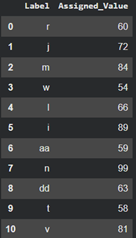
\includegraphics[width=0.3\linewidth]{figures/encouding_credit.png}
        \caption{ Encoding.}
        \label{}
      \end{minipage}
The union operation of all the letters in the dataframe is performed. A non-repeating random number is assigned using the size of the set. The encoding stays like this. Then it is normalized. We will stick with the Random Forest, which was calculated in the previous assignments and serves as the baseline model. \\
\vspace{0.15in}

% -------------------------------------------------

\noindent {\LARGE{\textbf{2. Performance Tables to Identify the Best}}} \
\vspace{0.5cm}

\noindent All metrics are reported as mean $\pm$ std over stratified 10-fold cross-validation.
\vspace{0.5cm}

\noindent {\Large{\textbf{A.} \textbf{The Hand-Written Digits Recognition Dataset}}}\\

\begin{table}[H]
\centering
\small
\caption{Hand-written Digits --- Random Forest performance (stratified 10-fold CV; \texttt{max\_depth=10}, \texttt{min\_size=2}, \texttt{min\_gain=0}).}
\label{tab:digits-rf}
\begin{tabular}{@{}lcccc@{}}
\toprule
Setting & Accuracy & Precision & Recall & F1 \\
\midrule
$\mathit{ntree}=1$  & $0.7963 \pm 0.0323$ & $0.8027 \pm 0.0319$ & $0.7962 \pm 0.0324$ & $0.7953 \pm 0.0326$ \\
$\mathit{ntree}=5$  & $0.9232 \pm 0.0173$ & $0.9266 \pm 0.0162$ & $0.9231 \pm 0.0176$ & $0.9232 \pm 0.0174$ \\
$\mathit{ntree}=10$ & $0.9616 \pm 0.0099$ & $0.9636 \pm 0.0092$ & $0.9615 \pm 0.0101$ & $0.9616 \pm 0.0099$ \\
$\mathit{ntree}=20$ & $0.9655 \pm 0.0063$ & $0.9668 \pm 0.0063$ & $0.9654 \pm 0.0064$ & $0.9654 \pm 0.0064$ \\
$\mathit{ntree}=30$ & $0.9672 \pm 0.0105$ & $0.9688 \pm 0.0097$ & $0.9671 \pm 0.0104$ & $0.9672 \pm 0.0103$ \\
$\mathit{ntree}=40$ & $0.9688 \pm 0.0090$ & $0.9703 \pm 0.0086$ & $0.9687 \pm 0.0090$ & $0.9687 \pm 0.0090$ \\
$\mathit{ntree}=50$ & $\mathbf{0.9739 \pm 0.0083}$ & $\mathbf{0.9748 \pm 0.0080}$ & $\mathbf{0.9738 \pm 0.0082}$ & $\mathbf{0.9738 \pm 0.0082}$ \\
\bottomrule
\end{tabular}
\end{table}

\begin{table}[H]
\centering
\small
\caption{Hand-written Digits --- k-NN with min-max normalization (stratified 10-fold CV; normalization fit on train fold and applied to test fold).}
\label{tab:digits-knn-norm}
\begin{tabular}{@{}lcccc@{}}
\toprule
Setting & Accuracy & Precision & Recall & F1 \\
\midrule
$k=1$  & $0.9872 \pm 0.0080$ & $0.9880 \pm 0.0073$ & $0.9871 \pm 0.0081$ & $0.9871 \pm 0.0080$ \\
$k=3$  & $\mathbf{0.9883 \pm 0.0102}$ & $\mathbf{0.9891 \pm 0.0093}$ & $\mathbf{0.9883 \pm 0.0103}$ & $\mathbf{0.9883 \pm 0.0102}$ \\
$k=5$  & $0.9883 \pm 0.0089$ & $0.9891 \pm 0.0080$ & $0.9883 \pm 0.0089$ & $0.9882 \pm 0.0089$ \\
$k=7$  & $0.9849 \pm 0.0094$ & $0.9858 \pm 0.0087$ & $0.9849 \pm 0.0095$ & $0.9848 \pm 0.0096$ \\
$k=9$  & $0.9816 \pm 0.0115$ & $0.9829 \pm 0.0102$ & $0.9814 \pm 0.0117$ & $0.9814 \pm 0.0117$ \\
$k=11$ & $0.9822 \pm 0.0106$ & $0.9836 \pm 0.0091$ & $0.9820 \pm 0.0108$ & $0.9820 \pm 0.0107$ \\
$k=15$ & $0.9799 \pm 0.0088$ & $0.9813 \pm 0.0077$ & $0.9797 \pm 0.0090$ & $0.9797 \pm 0.0089$ \\
$k=21$ & $0.9755 \pm 0.0107$ & $0.9769 \pm 0.0100$ & $0.9753 \pm 0.0108$ & $0.9752 \pm 0.0109$ \\
$k=31$ & $0.9676 \pm 0.0105$ & $0.9695 \pm 0.0101$ & $0.9674 \pm 0.0106$ & $0.9674 \pm 0.0107$ \\
$k=51$ & $0.9560 \pm 0.0137$ & $0.9580 \pm 0.0137$ & $0.9559 \pm 0.0136$ & $0.9557 \pm 0.0139$ \\
\bottomrule
\end{tabular}
\end{table}

\begin{table}[H]
\centering
\small
\caption{Hand-written Digits --- k-NN on raw features (no normalization).}
\label{tab:digits-knn-raw}
\begin{tabular}{@{}lcccc@{}}
\toprule
Setting & Accuracy & Precision & Recall & F1 \\
\midrule
$k=1$  & $0.9883 \pm 0.0078$ & $0.9890 \pm 0.0072$ & $0.9882 \pm 0.0079$ & $0.9882 \pm 0.0078$ \\
$k=3$  & $\mathbf{0.9888 \pm 0.0094}$ & $\mathbf{0.9896 \pm 0.0085}$ & $\mathbf{0.9888 \pm 0.0095}$ & $\mathbf{0.9888 \pm 0.0094}$ \\
$k=5$  & $0.9877 \pm 0.0093$ & $0.9886 \pm 0.0084$ & $0.9877 \pm 0.0094$ & $0.9877 \pm 0.0094$ \\
$k=7$  & $0.9855 \pm 0.0084$ & $0.9863 \pm 0.0079$ & $0.9855 \pm 0.0085$ & $0.9854 \pm 0.0086$ \\
$k=9$  & $0.9833 \pm 0.0094$ & $0.9844 \pm 0.0086$ & $0.9831 \pm 0.0095$ & $0.9830 \pm 0.0095$ \\
$k=11$ & $0.9839 \pm 0.0081$ & $0.9850 \pm 0.0072$ & $0.9837 \pm 0.0083$ & $0.9837 \pm 0.0082$ \\
$k=15$ & $0.9805 \pm 0.0072$ & $0.9819 \pm 0.0060$ & $0.9803 \pm 0.0074$ & $0.9803 \pm 0.0073$ \\
$k=21$ & $0.9760 \pm 0.0106$ & $0.9775 \pm 0.0096$ & $0.9758 \pm 0.0107$ & $0.9758 \pm 0.0108$ \\
$k=31$ & $0.9671 \pm 0.0110$ & $0.9690 \pm 0.0106$ & $0.9669 \pm 0.0111$ & $0.9668 \pm 0.0112$ \\
$k=51$ & $0.9565 \pm 0.0129$ & $0.9586 \pm 0.0127$ & $0.9564 \pm 0.0129$ & $0.9562 \pm 0.0131$ \\
\bottomrule
\end{tabular}
\end{table}

\begin{table}[H]
\centering
\small
\caption{Hand-written Digits --- best hyperparameter per algorithm (highest accuracy).}
\label{tab:digits-headline}
\begin{tabular}{@{}llcc@{}}
\toprule
Algorithm & Best setting & Accuracy & F1 \\
\midrule
Random Forest          & $\mathit{ntree}=50$       & $0.9739 \pm 0.0083$ & $0.9738 \pm 0.0082$ \\
k-NN (normalized)      & $k=3$                     & $0.9883 \pm 0.0102$ & $0.9883 \pm 0.0102$ \\
k-NN (raw)             & $k=3$                     & $\mathbf{0.9888 \pm 0.0094}$ & $\mathbf{0.9888 \pm 0.0094}$ \\
\bottomrule
\end{tabular}
\end{table}

    \begin{minipage}{\linewidth}
        \captionsetup{type=figure}
        \centering
        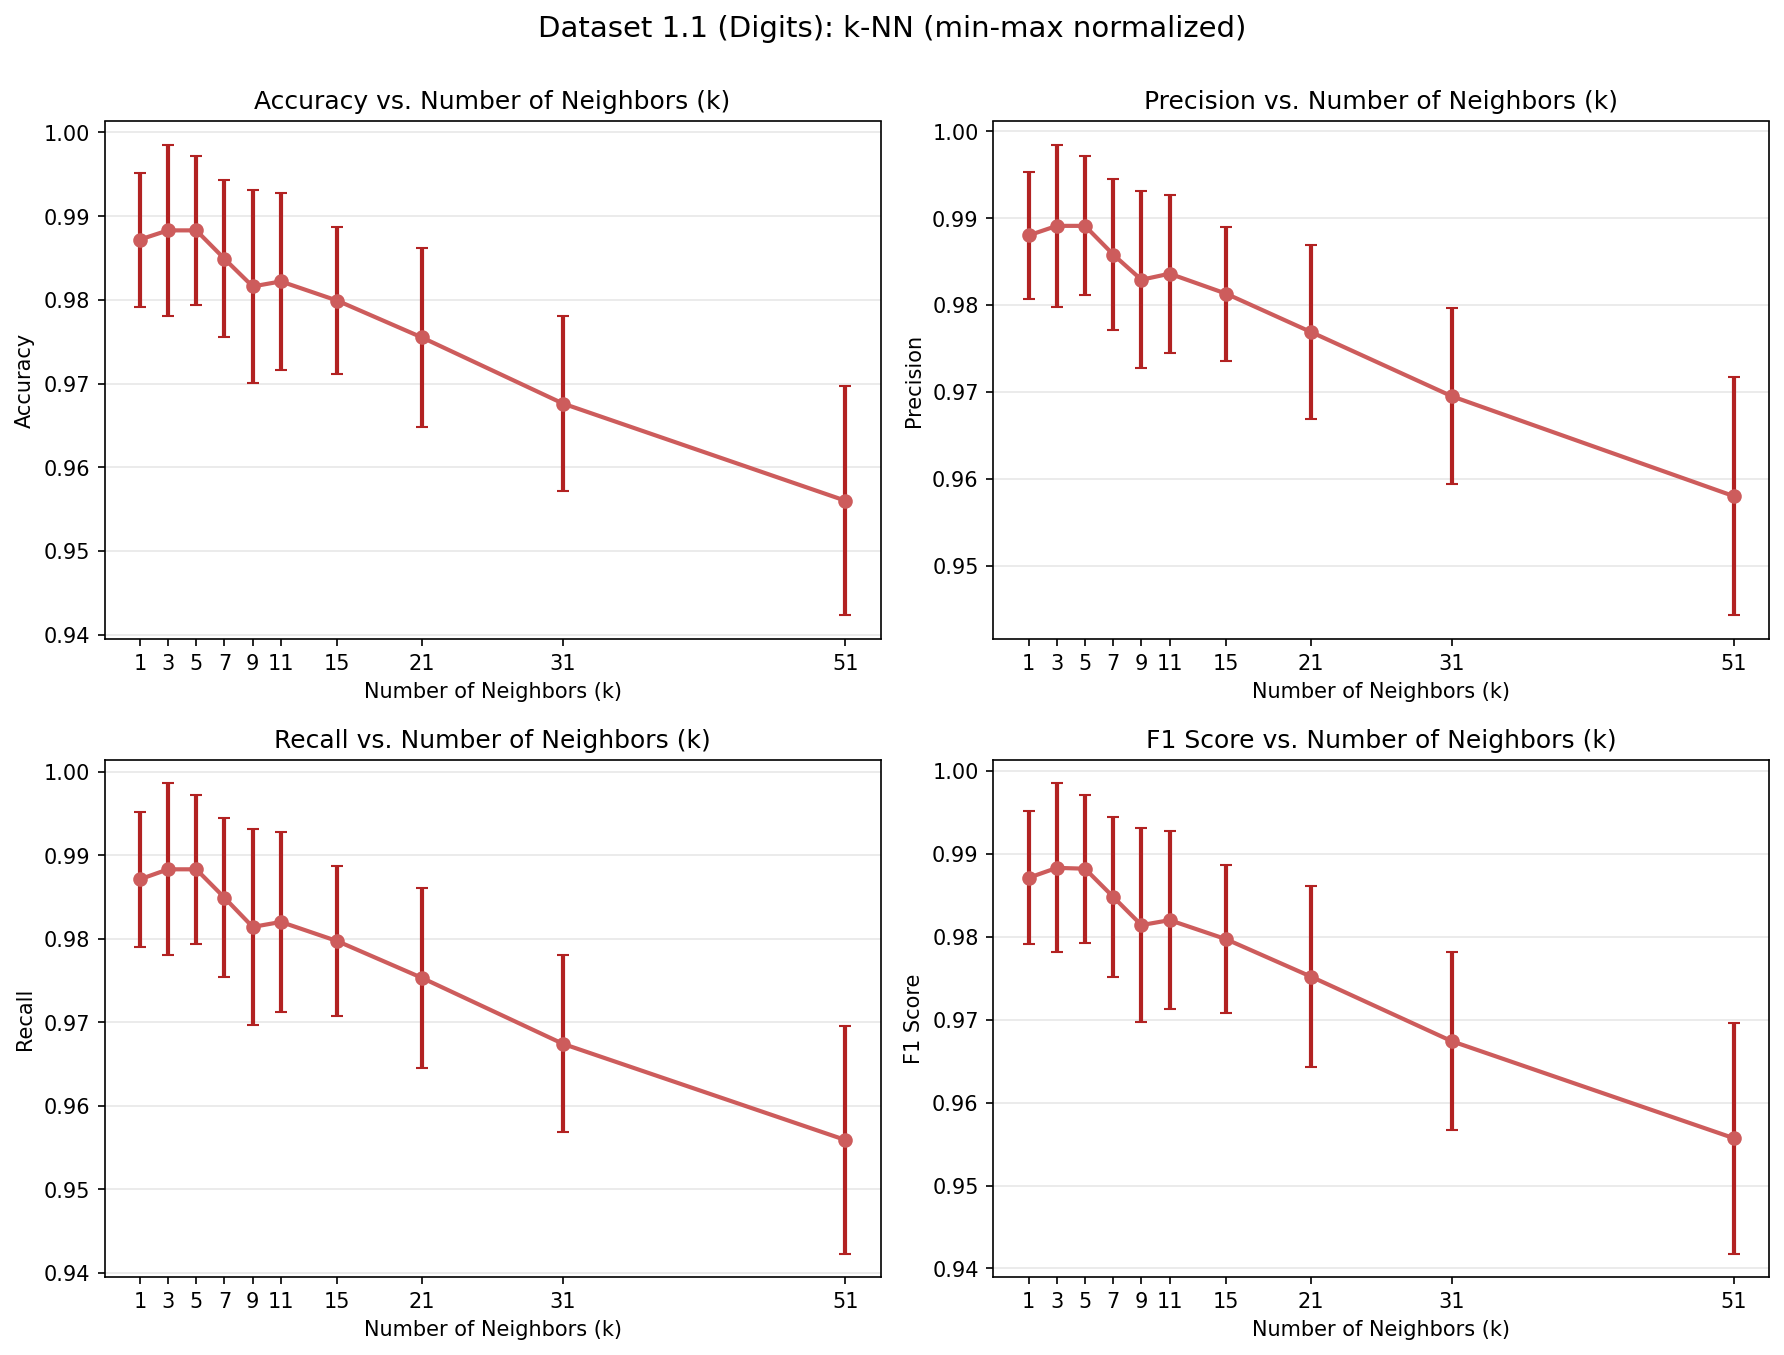
\includegraphics[width=0.8\linewidth]{figures/digits_knn_metrics.png}
        \caption{ k-NN Performance over Hand-written Digits.}
        \label{}
    \end{minipage}

    \begin{minipage}{\linewidth}
        \captionsetup{type=figure}
        \centering
        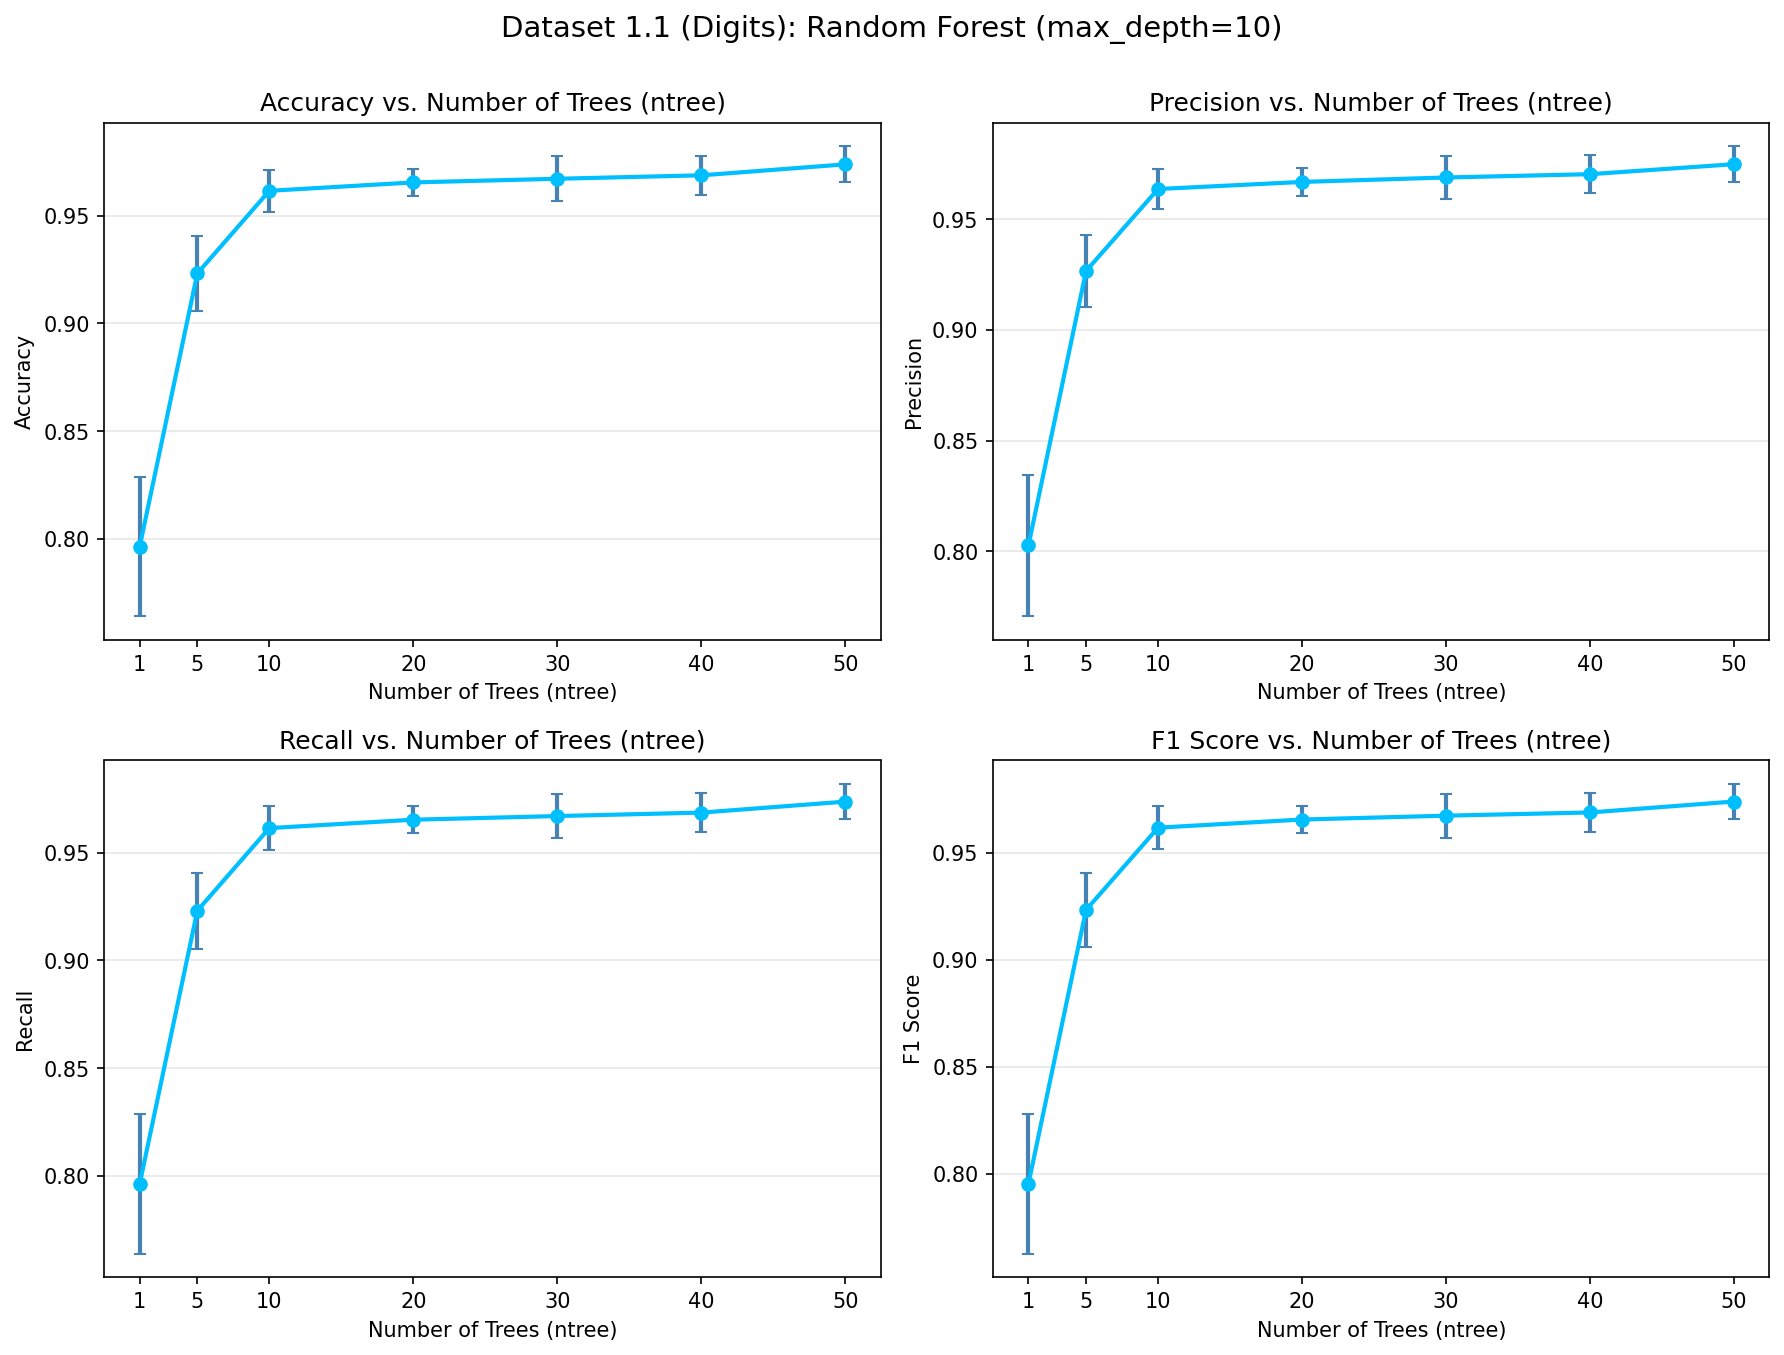
\includegraphics[width=0.8\linewidth]{figures/digits_rf_metrics.png}
        \caption{ Random Forest Performance over Hand-written Digits.}
        \label{}
    \end{minipage}

\begin{minipage}{\linewidth}
        \captionsetup{type=figure}
        \centering
        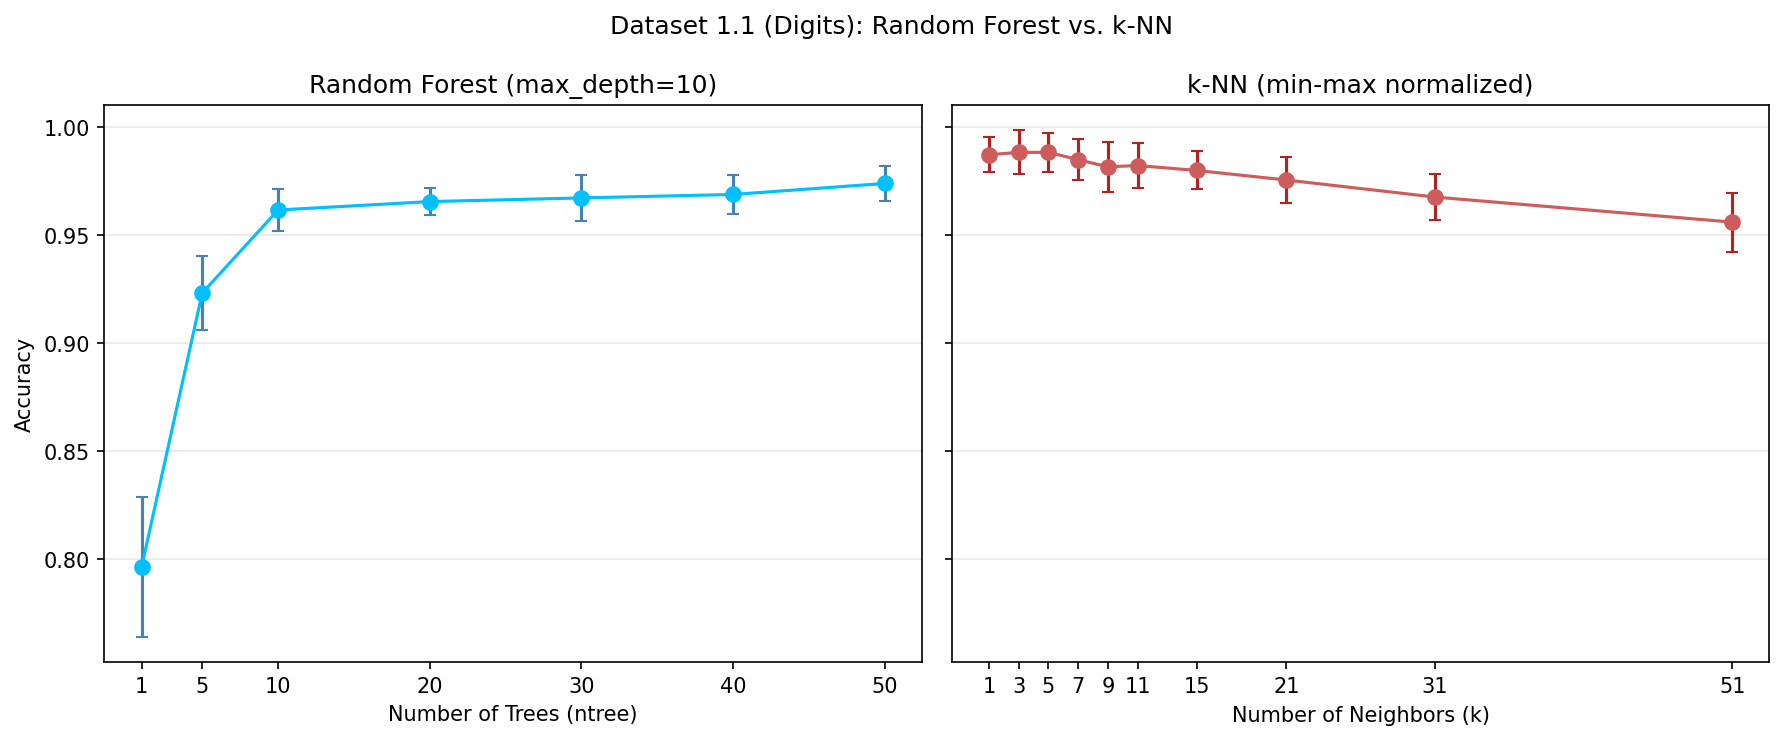
\includegraphics[width=0.8\linewidth]{figures/digits_comparison_rf_vs_knn.png}
        \caption{ Comparison of k-NN and RF over Hand-written Digits.}
        \label{}
    \end{minipage}

\noindent {\Large{\textbf{B.} \textbf{ The Oxford Parkinson’s Disease Detection Dataset}}}
\vspace{0.3cm}

{\Large\textbf{Neural Networks:}}\\
\vspace{0.3cm}

\noindent \textbf{Question 2.}You should evaluate the performance of each algorithm on a given dataset in terms of its accuracy and F1-score. Use stratified cross-validation with k = 10.


\vspace{0.3cm}
\noindent \textbf{Answer:}\\
\vspace{0.3cm}
\textbf{Neural Networks:}
\begin{enumerate}
    \item I evaluated neural network models with various architectures consisting of 1, 2, 3, and 4 hidden layers. The  number of neurons per layer was varied among 2, 4, 8, and 16.
    \item Stratified cross-validation with $k = 10$ was used to evaluate model performance.
    \item Various values of regularization parameter $\lambda$ were used to evaluate models performance such as $\{0, 0.1, 0.01\}$
    \item Different values of stopping criteria were used to evaluate the performance metrics such as $m$ in $\{1000, 2000, 3000\}$
    \item Multiple step size values $\alpha$ were used to evaluate the performance metrics such as $\{0.1, 0.05, 0.025, 0.075, 0.01\}$.
\end{enumerate}

\vspace{0.3cm}

\noindent \textbf{Question 3.} To achieve the best performance possible, you should carefully adjust the hyperparameters of each algorithm when deployed on a dataset. For example, you may have to experiment with different values of k when optimizing the k-NN algorithm; different values of ntree when optimizing a Random Forest; different architectures and regularization parameters when optimizing a neural network; etc.\\

\noindent \textbf{Answer:}\\

\textbf{Neural Networks:}

\begin{enumerate}

\item \textbf{Round 1 analysis}

\begin{enumerate}

\item For the Parkinsons disease detection dataset, I initially evaluated the neural network model with multiple hidden layers and varying the number of neurons per layer:

\begin{itemize}
    \item 1 hidden layer: [22, 2, 1], [22, 16, 1]
    \item 2 hidden layers: [22, 4, 8, 1], [22, 8, 16, 1], [22, 16, 32, 1]
    \item 3 hidden layers: [22, 4, 8, 16, 1]
    \item 4 hidden layers: [22, 2, 2, 2, 2, 1], [22, 2, 4, 8, 16, 1]
\end{itemize}

\item The regularization parameter $\lambda$ used for the neural network takes the value : $[0, 0.1, 0.01]$
\item The Stratified Cross Validation technique used for evaluation is $K = 10$ (stratified 10-fold cross-validation)
\item The stopping criterion used is a constant, pre-defined number of iterations $(m = 1000)$
\item The step size used is $\alpha = 0.1$ \\

Based on the above hyperparameters, the neural network model achieved the highest accuracy of 0.838099 for the architecture [22,16,32,1] with $\lambda = 0$, $\alpha = 0.1$, $m = 1000$
In contrast, the highest F1-score of 0.900901 was obtained for the architecture [22,2,1] with $\lambda$ = 0.1, $\alpha$ = 0.1, $m = 1000$.\\

To further improve performance, the same architectures and $\lambda$ values were evaluated with higher number of iterations $m = 2000$ and reduced step size $\alpha = 0.05$\\

\end{enumerate}

\item \textbf{Round 2 analysis}

\begin{enumerate}
\item The same neural network architectures and regularization parameters ($\lambda$) as described in Round 1 were used. However, different stopping criteria and step sizes were applied.
\item The stopping criterion used is a constant, pre-defined number of iterations $(m = 2000)$
\item The step size used is $\alpha = 0.05$ \\

\end{enumerate}

Based on the above hyperparameters, the neural network model achieved the highest accuracy of 0.856988 and the highest F1-Score of 0.914565 for the architecture [22,2,1] with $\lambda = 0.01$, $\alpha = 0.05$ and $m = 2000$.\\

Based on the results from Round 1 and Round 2, it can be observed that the performance metrics for more complex architectures with three or four hidden layers, such as [22,4,8,16,1], [22,2,2,2,2,1], and [22,2,4,8,16,1] stagnate and do not improve across different combinations of stopping criteria $m$, step size $\alpha$ and regularization parameters $\lambda$. This indicates that using more complex models with three or four hidden layers, even with varying number of neurons in each layer does not result in better performance for the Parkinson's Disease Detection dataset.\\

As a result, for the next round of analysis, I will avoid using these complex architectures and continue performance metrics analysis on simple architectures with one or two hidden layers, varying the number of neurons in each layer. Additionally, I will use stopping criteria of $m = 2000$ and step size $\alpha = 0.05$, as these hyper-parameters resulted in higher performance metric values for Accuracy and F-Score in Round 2 analysis compared to Round 1.\\


\item \textbf{Round 3 analysis}
\begin{enumerate}
\item In Round 3 analysis, the focus was on neural network architectures with one or two hidden layers with varying number of neurons in each layer

\begin{itemize}
    \item 1 hidden layer: [22, 3, 1], [22, 4, 1], [22, 8, 1]
    \item 2 hidden layers: [22, 2, 2, 1], [22, 2, 4, 1], [22, 2, 8, 1], [22, 2, 16, 1]

\end{itemize}
\item The same regularization parameter $\lambda$ used for the neural network takes the value : $[0, 0.1, 0.01]$
\item The stopping criterion used is a constant, pre-defined number of iterations $(m = 2000)$
\item The step size used is $\alpha = 0.05$ \\


\end{enumerate}

Based on the above hyperparameters, the neural network model achieved the highest accuracy of 0.866696 and the highest F1-Score of 0.919369 for the architecture [22,3,1] with $\lambda = 0.01$, $\alpha = 0.05$, and $m = 2000$. \\

Based on the results from Round 3, it can be observed that the performance metrics for architectures with two hidden layers, such as [22,2,2,1], [22,2,4,1], and [22,2,8,1] stagnate and show little or no improvement across different combinations of stopping criteria $m$, step size $\alpha$ and regularization parameters $\lambda$. \\

Based on the analysis from the three rounds, it can be observed that simple architectures with one hidden layer and fewer neurons in the hidden layer such as [22, 2, 1] and [22, 3, 1] achieved better performance metrics. This indicates that simpler models provide better generalization for the Parkinson's Disease Detection dataset.\\

\item \textbf{Round 4 analysis}
\begin{enumerate}

\item In Round 4 analysis, the focus was on neural network architectures with one and two hidden layers, which achieved higher accuracy and F1-scores in earlier rounds.

\begin{itemize}
    \item 1 hidden layer: [22, 2, 1], [22, 3, 1] with regularization parameter $\lambda$ : $0.01$
    \item 2 hidden layer: [22, 8, 16, 1] with regularization parameter $\lambda$ : $0.0$

\end{itemize}
\item The stopping criterion used is a constant, pre-defined number of iterations $(m = 2000)$
\item The step size $\alpha$ takes values in $\{0.1, 0.025, 0.075, 0.01\}$.\\


\end{enumerate}

The results for the above high performing architectures, using different new values of the step size hyperparameter $\alpha$ $\{0.1, 0.025, 0.075, 0.01\}$, resulted in lower accuracy and F1-Score compared to previous rounds, indicating that these step size values did not improve the performance of the model for these high-performing architectures as expected.\\

\item \textbf{Round 5 analysis}
\begin{enumerate}
\item In Round 5 analysis, the focus was on the best-performing neural network architecture, evaluated using a higher stopping criteria $(m = 3000)$.

\begin{itemize}
    \item 1 hidden layer: [22, 3, 1] with regularization parameter $\lambda$ : $0.01$

\end{itemize}
\item The stopping criterion used is a constant, pre-defined number of iterations $(m = 3000)$
\item The step size used is $\alpha = 0.05$\\

\end{enumerate}

The accuracy and F1-Score for the higher stopping criterion $(m = 3000)$ are lower compared to the earlier stopping criterion $(m = 2000)$. This indicates that increasing the number of iterations did not improve the models performance for the best performing architecture identified during earlier rounds of analysis.

\vspace{0.3cm}

\noindent \textbf{Question 4.} Given the above observation, you should first show, in a table, the performance of each algorithm (on a given dataset) under a few selected hyperparameters. You should evaluate at least 6 hyper-parameter settings. After analyzing the performance of each algorithm under different hyperparameters, identify the best hyperparameter setting, that is, the set of hyperparameters that resulted in the best performance for the corresponding algorithm on a particular dataset.\\

\noindent \textbf{Answer:}\\

\textbf{Round 1 analysis}

In Round 1, the neural network model achieved the highest accuracy of 0.838099 for the architecture [22,16,32,1] with $\lambda = 0$, $\alpha = 0.1$, $m = 1000$. \\

The neural network model achieved the highest F1-score of 0.900901 for the architecture [22,2,1] with $\lambda = 0.1$, $\alpha = 0.1$, $m = 1000$.\\

It can be observed that the performance metrics for more complex architectures with three or four hidden layers, such as [22,4,8,16,1], [22,2,2,2,2,1], and [22,2,4,8,16,1], stagnate and do not improve for the selected hyper-parameters. The accuracy value for these architectures remains constant at 0.754240, while the F1-Score value remains constant at 0.859848.\\

Simple architecture with one hidden layer generalizes well for the provided hyperparameter values. Both the [22,2,1] and [22,16,1] architecture achieves good accuracy and F1-score performance metrics.\\

Increasing the number of neurons in architectures with two hidden layers improves the performance of the neural network model and enhances generalization. For example, the [22,16,32,1] architecture performs better than [22,4,8,1].


\begin{table}[H]
\centering
\large
\renewcommand{\arraystretch}{1.3}
\setlength{\tabcolsep}{8pt}


\begin{tabular}{|c|c|c|c|c|c|}
\hline
\textbf{Architecture} & \textbf{$\lambda$} & \textbf{$\alpha$} & \textbf{$m$} & \textbf{Accuracy} & \textbf{F1-score} \\
\hline
$[22, 2, 1]$ & 0    & 0.1 & 1000 & 0.825058 & 0.894818 \\ \hline
\textbf{[22, 2, 1]} & \textbf{0.1}  & \textbf{0.1} & \textbf{1000} & 0.835322 & \textbf{0.900901} \\ \hline
$[22, 2, 1]$ & 0.01 & 0.1 & 1000 & 0.789795 & 0.874638 \\ \hline

$[22, 16, 1]$ & 0    & 0.1 & 1000 & 0.818392 & 0.885584 \\ \hline
$[22, 16, 1]$ & 0.1  & 0.1 & 1000 & 0.832807 & 0.896088 \\ \hline
$[22, 16, 1]$ & 0.01 & 0.1 & 1000 & 0.833070 & 0.895904 \\ \hline

$[22, 4, 8, 1]$ & 0    & 0.1 & 1000 & 0.764240 & 0.865043 \\ \hline
$[22, 4, 8, 1]$ & 0.1  & 0.1 & 1000 & 0.789795 & 0.878038 \\ \hline
$[22, 4, 8, 1]$ & 0.01 & 0.1 & 1000 & 0.794240 & 0.880225 \\ \hline

$[22, 8, 16, 1]$ & 0    & 0.1 & 1000 & 0.825322 & 0.893867 \\ \hline
$[22, 8, 16, 1]$ & 0.1  & 0.1 & 1000 & 0.830351 & 0.897188 \\ \hline
$[22, 8, 16, 1]$ & 0.01 & 0.1 & 1000 & 0.819795 & 0.891655 \\ \hline

\textbf{[22, 16, 32, 1]} & \textbf{0}    & \textbf{0.1} & \textbf{1000} & \textbf{0.838099} & 0.897959 \\ \hline
$[22, 16, 32, 1]$ & 0.1  & 0.1 & 1000 & 0.825614 & 0.889542 \\ \hline
$[22, 16, 32, 1]$ & 0.01 & 0.1 & 1000 & 0.831696 & 0.894620 \\ \hline

$[22, 4, 8, 16, 1]$ & 0    & 0.1 & 1000 & 0.764240 & 0.865043 \\ \hline
$[22, 4, 8, 16, 1]$ & 0.1  & 0.1 & 1000 & 0.754240 & 0.859848 \\ \hline
$[22, 4, 8, 16, 1]$ & 0.01 & 0.1 & 1000 & 0.754240 & 0.859848 \\ \hline

$[22, 2, 2, 2, 2, 1]$ & 0    & 0.1 & 1000 & 0.754240 & 0.859848 \\ \hline
$[22, 2, 2, 2, 2, 1]$ & 0.1  & 0.1 & 1000 & 0.754240 & 0.859848 \\ \hline
$[22, 2, 2, 2, 2, 1]$ & 0.01 & 0.1 & 1000 & 0.754240 & 0.859848 \\ \hline

$[22, 2, 4, 8, 16, 1]$ & 0    & 0.1 & 1000 & 0.754240 & 0.859848 \\ \hline
$[22, 2, 4, 8, 16, 1]$ & 0.1  & 0.1 & 1000 & 0.754240 & 0.859848 \\ \hline
$[22, 2, 4, 8, 16, 1]$ & 0.01 & 0.1 & 1000 & 0.754240 & 0.859848 \\ \hline

\end{tabular}
\caption{Round 1 Analysis : Performance metrics of all neural network architectures ($\lambda \in \{0, 0.1, 0.01\}$, $\alpha = 0.1$, $m = 1000$) using stratified 10-fold cross-validation}
\end{table}

\textbf{Round 2 analysis}

In Round 2, the neural network model achieved the highest accuracy of 0.856988 and the highest F1-score of 0.914565 for the architecture [22,2,1] with $\lambda = 0.01$, $\alpha = 0.1$, $m = 2000$. \\

It can be observed that the performance metrics for more complex architectures with three or four hidden layers, such as [22,4,8,16,1], [22,2,2,2,2,1], and [22,2,4,8,16,1], stagnate and do not improve for the selected hyper-parameters. The accuracy value for these architectures remains constant at 0.754240, while the F1-Score value remains constant at 0.859848.\\

Based on the observations, complex architectures with three or four hidden layers across various combinations of selected hyperparameters, do not generalize well for the Parkinson Disease detection dataset. \\

Simple architecture with one hidden layer generalizes well for the provided hyperparameter values. Both the [22,2,1] and [22,16,1] architecture achieves good accuracy and F1-score performance metrics.\\

Increasing the number of neurons in architectures with two hidden layers improves the performance of the neural network model and enhances generalization. For example, the [22,16,32,1] architecture performs better than [22,4,8,1].

\begin{table}[H]
\centering
\large
\renewcommand{\arraystretch}{1.3}
\setlength{\tabcolsep}{8pt}

\begin{tabular}{|c|c|c|c|c|c|}
\hline
\textbf{Architecture} & \textbf{$\lambda$} & \textbf{$\alpha$} & \textbf{$m$} & \textbf{Accuracy} & \textbf{F1-score} \\
\hline

$[22, 2, 1]$ & 0    & 0.05 & 2000 & 0.790877 & 0.876073 \\ \hline
$[22, 2, 1]$ & 0.1  & 0.05 & 2000 & 0.783684 & 0.873757 \\ \hline
\textbf{[22, 2, 1]} & \textbf{0.01} & \textbf{0.05} & \textbf{2000} & \textbf{0.856988} & \textbf{0.914565} \\ \hline

$[22, 16, 1]$ & 0    & 0.05 & 2000 & 0.831988 & 0.894811 \\ \hline
$[22, 16, 1]$ & 0.1  & 0.05 & 2000 & 0.830322 & 0.895631 \\ \hline
$[22, 16, 1]$ & 0.01 & 0.05 & 2000 & 0.824737 & 0.889840 \\ \hline

$[22, 4, 8, 1]$ & 0    & 0.05 & 2000 & 0.764240 & 0.865043 \\ \hline
$[22, 4, 8, 1]$ & 0.1  & 0.05 & 2000 & 0.781140 & 0.874167 \\ \hline
$[22, 4, 8, 1]$ & 0.01 & 0.05 & 2000 & 0.769795 & 0.866242 \\ \hline

$[22, 8, 16, 1]$ & 0    & 0.05 & 2000 & 0.846988 & 0.905541 \\ \hline
$[22, 8, 16, 1]$ & 0.1  & 0.05 & 2000 & 0.824795 & 0.893475 \\ \hline
$[22, 8, 16, 1]$ & 0.01 & 0.05 & 2000 & 0.831170 & 0.896094 \\ \hline

$[22, 16, 32, 1]$ & 0    & 0.05 & 2000 & 0.815322 & 0.883301 \\ \hline
$[22, 16, 32, 1]$ & 0.1  & 0.05 & 2000 & 0.827018 & 0.889883 \\ \hline
$[22, 16, 32, 1]$ & 0.01 & 0.05 & 2000 & 0.841462 & 0.899596 \\ \hline

$[22, 4, 8, 16, 1]$ & 0    & 0.05 & 2000 & 0.754240 & 0.859848 \\ \hline
$[22, 4, 8, 16, 1]$ & 0.1  & 0.05 & 2000 & 0.754240 & 0.859848 \\ \hline
$[22, 4, 8, 16, 1]$ & 0.01 & 0.05 & 2000 & 0.754240 & 0.859848 \\ \hline

$[22, 2, 2, 2, 2, 1]$ & 0    & 0.05 & 2000 & 0.754240 & 0.859848 \\ \hline
$[22, 2, 2, 2, 2, 1]$ & 0.1  & 0.05 & 2000 & 0.754240 & 0.859848 \\ \hline
$[22, 2, 2, 2, 2, 1]$ & 0.01 & 0.05 & 2000 & 0.754240 & 0.859848 \\ \hline

$[22, 2, 4, 8, 16, 1]$ & 0    & 0.05 & 2000 & 0.754240 & 0.859848 \\ \hline
$[22, 2, 4, 8, 16, 1]$ & 0.1  & 0.05 & 2000 & 0.754240 & 0.859848 \\ \hline
$[22, 2, 4, 8, 16, 1]$ & 0.01 & 0.05 & 2000 & 0.754240 & 0.859848 \\ \hline

\end{tabular}

\caption{Round 2 Analysis : Performance metrics of all neural network architectures ($\lambda \in \{0, 0.1, 0.01\}$, $\alpha = 0.05$, $m = 2000$) using stratified 10-fold cross-validation}
\end{table}



\textbf{Round 3 analysis}

In Round 3, the neural network model achieved the highest accuracy of 0.866696 and the highest F1-score of 0.919369 for the architecture [22,3,1] with $\lambda = 0.01$, $\alpha = 0.05$, $m = 2000$. \\

Simple architecture with one hidden layer generalizes well for the provided hyperparameter values. The [22,3,1], [22,4,1] and [22,8,1] architectures achieve good accuracy and F1-score performance.\\

It can be observed that the performance metrics for architectures with two hidden layers and varying numbers of neurons, such as [22,2,2,1], [22,2,4,1], and [22,2,8,1], stagnate and do not improve for the selected hyperparameters. The accuracy for these architectures remains constant at 0.754240, while the F1-score remains at 0.859848.\\

Only the two-hidden-layer architecture [22,2,16,1] shows moderate improvement in accuracy and F1-score, rather than stagnation.


\begin{table}[H]
\centering
\large
\renewcommand{\arraystretch}{1.2}
\setlength{\tabcolsep}{6pt}

\begin{tabular}{|c|c|c|c|c|c|}
\hline
\textbf{Architecture} & \textbf{$\lambda$} & \textbf{$\alpha$} & \textbf{$m$} & \textbf{Accuracy} & \textbf{F1-score} \\
\hline

$[22,3,1]$ & 0    & 0.05 & 2000 & 0.818947 & 0.888841 \\ \hline
$[22,3,1]$ & 0.1  & 0.05 & 2000 & 0.835585 & 0.902359 \\ \hline
\textbf{[22,3,1]} & \textbf{0.01} & \textbf{0.05} & \textbf{2000} & \textbf{0.866696} & \textbf{0.919369} \\ \hline

$[22,4,1]$ & 0    & 0.05 & 2000 & 0.842251 & 0.903289 \\ \hline
$[22,4,1]$ & 0.1  & 0.05 & 2000 & 0.842544 & 0.903355 \\ \hline
$[22,4,1]$ & 0.01 & 0.05 & 2000 & 0.813977 & 0.884707 \\ \hline

$[22,8,1]$ & 0    & 0.05 & 2000 & 0.836696 & 0.898814 \\ \hline
$[22,8,1]$ & 0.1  & 0.05 & 2000 & 0.830877 & 0.894862 \\ \hline
$[22,8,1]$ & 0.01 & 0.05 & 2000 & 0.835380 & 0.897151 \\ \hline

$[22,2,2,1]$ & 0    & 0.05 & 2000 & 0.754240 & 0.859848 \\ \hline
$[22,2,2,1]$ & 0.1  & 0.05 & 2000 & 0.754240 & 0.859848 \\ \hline
$[22,2,2,1]$ & 0.01 & 0.05 & 2000 & 0.754240 & 0.859848 \\ \hline

$[22,2,4,1]$ & 0    & 0.05 & 2000 & 0.754240 & 0.859848 \\ \hline
$[22,2,4,1]$ & 0.1  & 0.05 & 2000 & 0.754240 & 0.859848 \\ \hline
$[22,2,4,1]$ & 0.01 & 0.05 & 2000 & 0.754240 & 0.859848 \\ \hline

$[22,2,8,1]$ & 0    & 0.05 & 2000 & 0.754240 & 0.859848 \\ \hline
$[22,2,8,1]$ & 0.1  & 0.05 & 2000 & 0.769240 & 0.867884 \\ \hline
$[22,2,8,1]$ & 0.01 & 0.05 & 2000 & 0.764240 & 0.865043 \\ \hline

$[22,2,16,1]$ & 0    & 0.05 & 2000 & 0.769503 & 0.867695 \\ \hline
$[22,2,16,1]$ & 0.1  & 0.05 & 2000 & 0.764240 & 0.865043 \\ \hline
$[22,2,16,1]$ & 0.01 & 0.05 & 2000 & 0.799795 & 0.883454 \\ \hline

\end{tabular}

\caption{Round 3 Analysis : Performance metrics of all neural network architectures ($\lambda \in \{0, 0.1, 0.01\}$, $\alpha = 0.05$, $m = 2000$) using stratified 10-fold cross-validation}
\end{table}


\textbf{Round 4 analysis}

In Round 4 analysis, the focus was on neural network architectures with one and two hidden layers, which achieved higher accuracy and F1-scores in earlier rounds.

In Round 4, the neural network model achieved the highest accuracy of 0.840848 and the highest F1-score of 0.902125 for the architecture [22,2,1] with $\lambda = 0.01$, $\alpha = 0.075$, $m = 2000$. \\

The results for the selected high performing architectures, using different new values of the step size hyperparameter $\alpha \in \{0.1, 0.025, 0.075, 0.01\}$, resulted in lower accuracy and F1-Score compared to previous rounds, indicating that these step size values did not improve the performance of the model for these high-performing architectures as expected.\\

All three architectures exhibited above-average performance for the new step size hyperparameters.


\begin{table}[H]
\centering
\large
\renewcommand{\arraystretch}{1.3}
\setlength{\tabcolsep}{8pt}

\begin{tabular}{|c|c|c|c|c|c|}
\hline
\textbf{Architecture} & \textbf{$\alpha$} & \textbf{$\lambda$} & \textbf{$m$} & \textbf{Accuracy} & \textbf{F1-score} \\
\hline

% [22,2,1]
$[22,2,1]$ & 0.1   & 0.01 & 2000 & 0.816959 & 0.888299 \\ \hline
$[22,2,1]$ & 0.025 & 0.01 & 2000 & 0.769795 & 0.867866 \\ \hline
\textbf{[22,2,1]} & \textbf{0.075} & \textbf{0.01} & \textbf{2000} & \textbf{0.840848} & \textbf{0.902125} \\ \hline
$[22,2,1]$ & 0.01  & 0.01 & 2000 & 0.754240 & 0.859848 \\ \hline

% [22,3,1]
$[22,3,1]$ & 0.1   & 0.01 & 2000 & 0.829766 & 0.892389 \\ \hline
$[22,3,1]$ & 0.025 & 0.01 & 2000 & 0.759503 & 0.862500 \\ \hline
$[22,3,1]$ & 0.075 & 0.01 & 2000 & 0.826725 & 0.891123 \\ \hline
$[22,3,1]$ & 0.01  & 0.01 & 2000 & 0.754240 & 0.859848 \\ \hline

% NEW: [22,8,16,1]
$[22,8,16,1]$ & 0.1   & 0.0 & 2000 & 0.831959 & 0.893957 \\ \hline
$[22,8,16,1]$ & 0.025 & 0.0 & 2000 & 0.765351 & 0.865682 \\ \hline
$[22,8,16,1]$ & 0.075 & 0.0 & 2000 & 0.830877 & 0.893226 \\ \hline
$[22,8,16,1]$ & 0.01  & 0.0 & 2000 & 0.754240 & 0.859848 \\ \hline

\end{tabular}

\caption{Round 4 Analysis : Performance metrics of top performing neural network architectures ($\lambda \in \{0.01, 0.0\}$, $\alpha \in \{0.1, 0.025, 0.075, 0.01\}$, $m = 2000$) using stratified 10-fold cross-validation}
\end{table}

\textbf{Round 5 analysis}

In Round 5 analysis, the focus was on the best-performing neural network architecture [22,3,1], evaluated using a higher stopping criterion ($m = 3000$). The accuracy and F1-score for the higher stopping criterion ($m = 3000$) are lower compared to the earlier setting ($m = 2000$). This indicates that increasing the number of iterations did not improve the model’s performance for the best-performing architecture identified in the earlier rounds of analysis.

\begin{table}[H]
\centering
\large
\renewcommand{\arraystretch}{1.3}
\setlength{\tabcolsep}{8pt}

\begin{tabular}{|c|c|c|c|c|c|}
\hline
\textbf{Architecture} & \textbf{$\alpha$} & \textbf{$\lambda$} & \textbf{$m$} & \textbf{Accuracy} & \textbf{F1-score} \\
\hline

$[22,3,1]$ & 0.05 & 0.01 & 3000 & 0.835614 & 0.897459 \\ \hline

\end{tabular}

\caption{Round 5 Analysis : Performance metrics of highest performing neural network architecture [22, 3, 1] with hyperparameters ($\lambda \in \{0.01\}$, $\alpha \in \{0.05\}$, $m = 3000$) using stratified 10-fold cross-validation}
\end{table}

\large{\textbf{Best Hyperparameter Setting for Neural Network Algorithm}} \\

\vspace{0.3cm}

\textbf{The best hyperparameter setting for the Neural Network algorithm is architecture $[22, 3, 1]$ with regularization parameter $\lambda = 0.01$, step size $\alpha = 0.05$, and stopping criteria
$m = 2000$ iterations, achieving the highest accuracy of \textbf{0.866696} and F1-Score of \textbf{0.919369} on the Oxford Parkinson's Disease Detection Dataset.}

\begin{table}[H]
\centering
\large
\renewcommand{\arraystretch}{1.5}
\setlength{\tabcolsep}{15pt}
\begin{tabular}{|c|c|c|c|c|c|}
\hline
\textbf{Architecture} & \textbf{$\alpha$} & \textbf{$\lambda$} & \textbf{$m$} & \textbf{Accuracy} & \textbf{F1-Score} \\
\hline
\textbf{[22, 3, 1]} & \textbf{0.05} & \textbf{0.01} & \textbf{2000} & \textbf{0.866696} & \textbf{0.919369} \\
\hline
\end{tabular}
\caption{Best Hyperparameter Setting for the Neural Network Algorithm
on the Oxford Parkinson's Disease Detection Dataset}
\label{tab:nn_best_parkinsons}
\end{table}

\end{enumerate}

{\Large\textbf{K-Nearest-Neighbor Algorithm:}}\\
\vspace{0.3cm}

\noindent \textbf{Question 2.}You should evaluate the performance of each algorithm on a given dataset in terms of its accuracy and F1-score. Use stratified cross-validation with k = 10.

\vspace{0.3cm}
\noindent \textbf{Answer:}\\

\textbf{K-Nearest-Neighbor Algorithm:}
\begin{enumerate}
    \item I evaluated the k-NN model for values of $k$ ranging from 1 to 51, considering only odd values (1, 3, 5, \ldots, 51).
    \item Stratified cross-validation with $k = 10$ was used to evaluate model performance.
    \item Each value of $k$ was evaluated 20 times using a shuffled dataset to ensure that the order in which examples appear in the dataset does not affect the learning process\\
\end{enumerate}

\noindent \textbf{Question 3.} To achieve the best performance possible, you should carefully adjust the hyperparameters of each algorithm when deployed on a dataset. For example, you may have to experiment with different values of k when optimizing the k-NN algorithm; different values of ntree when optimizing a Random Forest; different architectures and regularization parameters when optimizing a neural network; etc.\\

\noindent \textbf{Answer:}\\

\vspace{0.3cm}
\textbf{K-Nearest-Neighbor Algorithm:}

\vspace{0.3cm}

To achieve the best performance, the hyperparameter $k$ was systematically tuned for the k-NN algorithm.

Different values of $k$ ranging from 1 to 51 were evaluated, considering only odd values (1, 3, 5, \ldots, 51) to avoid ties during classification.

The best $k$ value was selected based on the highest accuracy and F1-score value for running the K-NN model for various values of $k$
\\

\vspace{0.3cm}

\noindent \textbf{Question 4.} Given the above observation, you should first show, in a table, the performance of each algorithm (on a given dataset) under a few selected hyperparameters. You should evaluate at least 6 hyper-parameter settings. After analyzing the performance of each algorithm under different hyperparameters, identify the best hyperparameter setting, that is, the set of hyperparameters that resulted in the best performance for the corresponding algorithm on a particular dataset.\\

\vspace{0.3cm}
\noindent \textbf{Answer:}\\

\vspace{0.3cm}

\begin{table}[H]
\large
\centering
\begin{tabular}{|c|c|c|}
\hline
\textbf{k} & \textbf{Test Accuracy} & \textbf{Test F1-score} \\
\hline
\textbf{1}  & \textbf{0.958731} & \textbf{0.972024} \\ \hline
3  & 0.933386 & 0.955362 \\ \hline
5  & 0.929589 & 0.953452 \\ \hline
7  & 0.917371 & 0.946224 \\ \hline
9  & 0.906712 & 0.940283 \\ \hline
11 & 0.891402 & 0.930989 \\ \hline
13 & 0.871067 & 0.919622 \\ \hline
15 & 0.849937 & 0.908039 \\ \hline
17 & 0.829114 & 0.896883 \\ \hline
19 & 0.826117 & 0.895915 \\ \hline
21 & 0.824823 & 0.895672 \\ \hline
23 & 0.825456 & 0.896434 \\ \hline
25 & 0.826192 & 0.896955 \\ \hline
27 & 0.828088 & 0.898196 \\ \hline
29 & 0.831940 & 0.900322 \\ \hline
31 & 0.832130 & 0.900597 \\ \hline
33 & 0.835532 & 0.902399 \\ \hline
35 & 0.838493 & 0.903870 \\ \hline
37 & 0.837021 & 0.903151 \\ \hline
39 & 0.828843 & 0.898603 \\ \hline
41 & 0.824997 & 0.896673 \\ \hline
43 & 0.813095 & 0.890141 \\ \hline
45 & 0.814993 & 0.891311 \\ \hline
47 & 0.804863 & 0.885745 \\ \hline
49 & 0.796088 & 0.881299 \\ \hline
51 & 0.787721 & 0.876934 \\ \hline
\end{tabular}
\caption{Test performance of k-NN for different values of $k$}
\end{table}


For $K = 3$ and $K = 5$, the K-NN model achieves peak performance with better generalization compared to $K = 1$. These values of $K$ effectively capture the underlying patterns correctly and makes higher accuracy and F1-score predictions in the Parkinson's Disease Detection dataset.

\vspace{0.3cm}
For $K = 1$, the model achieves highest test accuracy (0.958731) and F1-Score (0.972024). The model is overfitting to training data. If one of the neighbors is incorrect, it results in incorrect prediction. The model is highly sensitive to outliers and noise.

\vspace{0.3cm}

\large{\textbf{Best Hyperparameter Setting for the K-Nearest-Neighbor Algorithm}} \\
\vspace{0.3cm}

\textbf{The best hyperparameter setting for the K-Nearest-Neighbor algorithm
is $k = 1$, achieving the highest accuracy of \textbf{0.958731} and
F1-Score of \textbf{0.972024} on the Oxford Parkinson's Disease
Detection Dataset.}

\begin{table}[H]
\centering
\large
\renewcommand{\arraystretch}{1.5}
\setlength{\tabcolsep}{20pt}
\begin{tabular}{|c|c|c|}
\hline
\textbf{Number of Nearest Neighbours (k)} & \textbf{Test Accuracy} & \textbf{Test F1-Score} \\
\hline
\textbf{1} & \textbf{0.958731} & \textbf{0.972024} \\
\hline
\end{tabular}
\caption{Best Hyperparameter Setting for the K-Nearest Neighbor
Algorithm on the Oxford Parkinson's Disease Detection Dataset}
\label{tab:knn_best_parkinsons}
\end{table}


\vspace{0.3cm}


\noindent {\Large{\textbf{C.} \textbf{ The Rice Grains Dataset}}}\\

\begin{table}[H]
\centering
\small
\caption{Rice Varieties --- Random Forest performance (stratified 10-fold CV; \texttt{max\_depth=5}, \texttt{min\_size=2}, \texttt{min\_gain=0}).}
\label{tab:rice-rf}
\begin{tabular}{@{}lcccc@{}}
\toprule
Setting & Accuracy & Precision & Recall & F1 \\
\midrule
$\mathit{ntree}=1$  & $0.9171 \pm 0.0198$ & $0.9169 \pm 0.0210$ & $0.9153 \pm 0.0180$ & $0.9153 \pm 0.0198$ \\
$\mathit{ntree}=5$  & $0.9257 \pm 0.0137$ & $0.9254 \pm 0.0143$ & $0.9230 \pm 0.0138$ & $0.9240 \pm 0.0140$ \\
$\mathit{ntree}=10$ & $0.9262 \pm 0.0121$ & $0.9257 \pm 0.0125$ & $0.9239 \pm 0.0124$ & $0.9245 \pm 0.0123$ \\
$\mathit{ntree}=20$ & $0.9255 \pm 0.0139$ & $0.9249 \pm 0.0145$ & $0.9230 \pm 0.0140$ & $0.9237 \pm 0.0142$ \\
$\mathit{ntree}=30$ & $0.9265 \pm 0.0135$ & $0.9259 \pm 0.0143$ & $0.9243 \pm 0.0132$ & $0.9248 \pm 0.0137$ \\
$\mathit{ntree}=40$ & $\mathbf{0.9283 \pm 0.0152}$ & $\mathbf{0.9278 \pm 0.0161}$ & $\mathbf{0.9261 \pm 0.0148}$ & $\mathbf{0.9267 \pm 0.0154}$ \\
$\mathit{ntree}=50$ & $0.9260 \pm 0.0147$ & $0.9255 \pm 0.0152$ & $0.9236 \pm 0.0149$ & $0.9243 \pm 0.0150$ \\
\bottomrule
\end{tabular}
\end{table}

\begin{table}[H]
\centering
\small
\caption{Rice Varieties --- k-NN with min-max normalization (stratified 10-fold CV; normalization fit on train fold and applied to test fold).}
\label{tab:rice-knn-norm}
\begin{tabular}{@{}lcccc@{}}
\toprule
Setting & Accuracy & Precision & Recall & F1 \\
\midrule
$k=1$  & $0.8866 \pm 0.0153$ & $0.8848 \pm 0.0162$ & $0.8851 \pm 0.0157$ & $0.8843 \pm 0.0155$ \\
$k=3$  & $0.9123 \pm 0.0132$ & $0.9112 \pm 0.0141$ & $0.9102 \pm 0.0127$ & $0.9104 \pm 0.0133$ \\
$k=5$  & $0.9199 \pm 0.0161$ & $0.9192 \pm 0.0174$ & $0.9178 \pm 0.0155$ & $0.9182 \pm 0.0163$ \\
$k=7$  & $0.9215 \pm 0.0184$ & $0.9207 \pm 0.0196$ & $0.9193 \pm 0.0179$ & $0.9198 \pm 0.0187$ \\
$k=9$  & $0.9236 \pm 0.0158$ & $0.9228 \pm 0.0172$ & $0.9216 \pm 0.0151$ & $0.9219 \pm 0.0160$ \\
$k=11$ & $0.9241 \pm 0.0163$ & $0.9231 \pm 0.0176$ & $0.9224 \pm 0.0155$ & $0.9225 \pm 0.0165$ \\
$k=15$ & $0.9239 \pm 0.0146$ & $0.9234 \pm 0.0158$ & $0.9214 \pm 0.0142$ & $0.9221 \pm 0.0148$ \\
$k=21$ & $0.9270 \pm 0.0169$ & $0.9263 \pm 0.0177$ & $0.9248 \pm 0.0168$ & $0.9254 \pm 0.0172$ \\
$k=31$ & $0.9281 \pm 0.0167$ & $0.9275 \pm 0.0173$ & $0.9258 \pm 0.0168$ & $0.9264 \pm 0.0170$ \\
$k=51$ & $\mathbf{0.9289 \pm 0.0176}$ & $\mathbf{0.9282 \pm 0.0182}$ & $\mathbf{0.9268 \pm 0.0179}$ & $\mathbf{0.9273 \pm 0.0180}$ \\
\bottomrule
\end{tabular}
\end{table}

\begin{table}[H]
\centering
\small
\caption{Rice Varieties --- k-NN on raw features (no normalization).}
\label{tab:rice-knn-raw}
\begin{tabular}{@{}lcccc@{}}
\toprule
Setting & Accuracy & Precision & Recall & F1 \\
\midrule
$k=1$  & $0.8682 \pm 0.0201$ & $0.8660 \pm 0.0209$ & $0.8652 \pm 0.0205$ & $0.8653 \pm 0.0205$ \\
$k=3$  & $\mathbf{0.8890 \pm 0.0121}$ & $\mathbf{0.8889 \pm 0.0135}$ & $\mathbf{0.8844 \pm 0.0121}$ & $\mathbf{0.8860 \pm 0.0123}$ \\
$k=5$  & $0.8856 \pm 0.0140$ & $0.8862 \pm 0.0160$ & $0.8802 \pm 0.0134$ & $0.8824 \pm 0.0141$ \\
$k=7$  & $0.8832 \pm 0.0156$ & $0.8843 \pm 0.0186$ & $0.8773 \pm 0.0142$ & $0.8798 \pm 0.0156$ \\
$k=9$  & $0.8824 \pm 0.0156$ & $0.8843 \pm 0.0191$ & $0.8758 \pm 0.0146$ & $0.8788 \pm 0.0157$ \\
$k=11$ & $0.8816 \pm 0.0140$ & $0.8837 \pm 0.0153$ & $0.8748 \pm 0.0146$ & $0.8779 \pm 0.0145$ \\
$k=15$ & $0.8824 \pm 0.0130$ & $0.8850 \pm 0.0145$ & $0.8751 \pm 0.0137$ & $0.8785 \pm 0.0135$ \\
$k=21$ & $0.8835 \pm 0.0189$ & $0.8864 \pm 0.0205$ & $0.8760 \pm 0.0197$ & $0.8796 \pm 0.0197$ \\
$k=31$ & $0.8840 \pm 0.0172$ & $0.8880 \pm 0.0186$ & $0.8757 \pm 0.0183$ & $0.8798 \pm 0.0180$ \\
$k=51$ & $0.8835 \pm 0.0171$ & $0.8880 \pm 0.0194$ & $0.8749 \pm 0.0174$ & $0.8793 \pm 0.0177$ \\
\bottomrule
\end{tabular}
\end{table}

\begin{table}[H]
\centering
\small
\caption{Rice Varieties --- best hyperparameter per algorithm (highest accuracy).}
\label{tab:rice-headline}
\begin{tabular}{@{}llcc@{}}
\toprule
Algorithm & Best setting & Accuracy & F1 \\
\midrule
Random Forest          & $\mathit{ntree}=40$       & $0.9283 \pm 0.0152$ & $0.9267 \pm 0.0154$ \\
k-NN (normalized)      & $k=51$                    & $\mathbf{0.9289 \pm 0.0176}$ & $\mathbf{0.9273 \pm 0.0180}$ \\
k-NN (raw)             & $k=3$                     & $0.8890 \pm 0.0121$ & $0.8860 \pm 0.0123$ \\
\bottomrule
\end{tabular}
\end{table}

    \begin{minipage}{\linewidth}
        \captionsetup{type=figure}
        \centering
        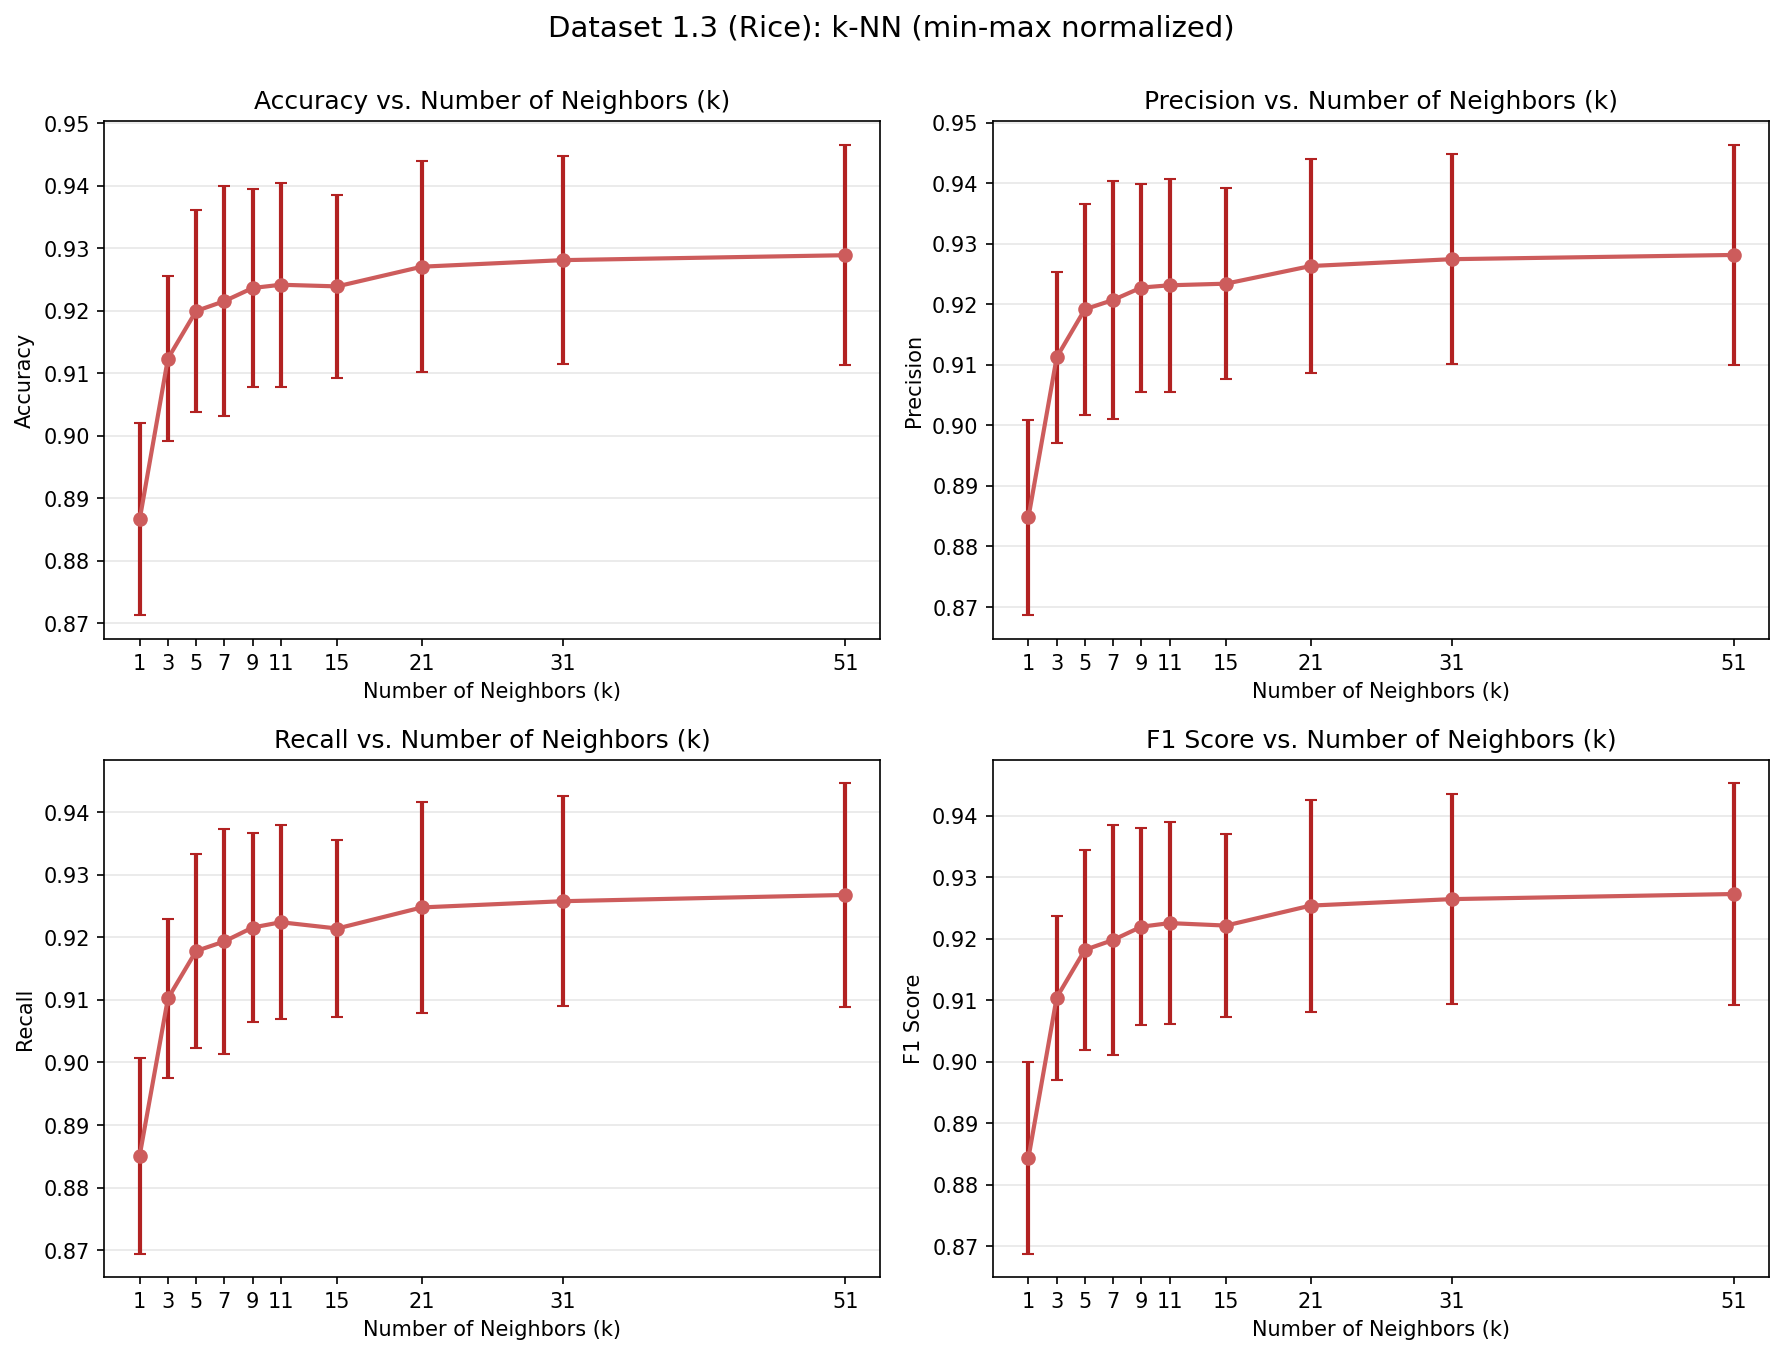
\includegraphics[width=0.8\linewidth]{figures/rice_knn_metrics.png}
        \caption{ k-NN Performance over Rice Varieties.}
        \label{}
    \end{minipage}

    \begin{minipage}{\linewidth}
        \captionsetup{type=figure}
        \centering
        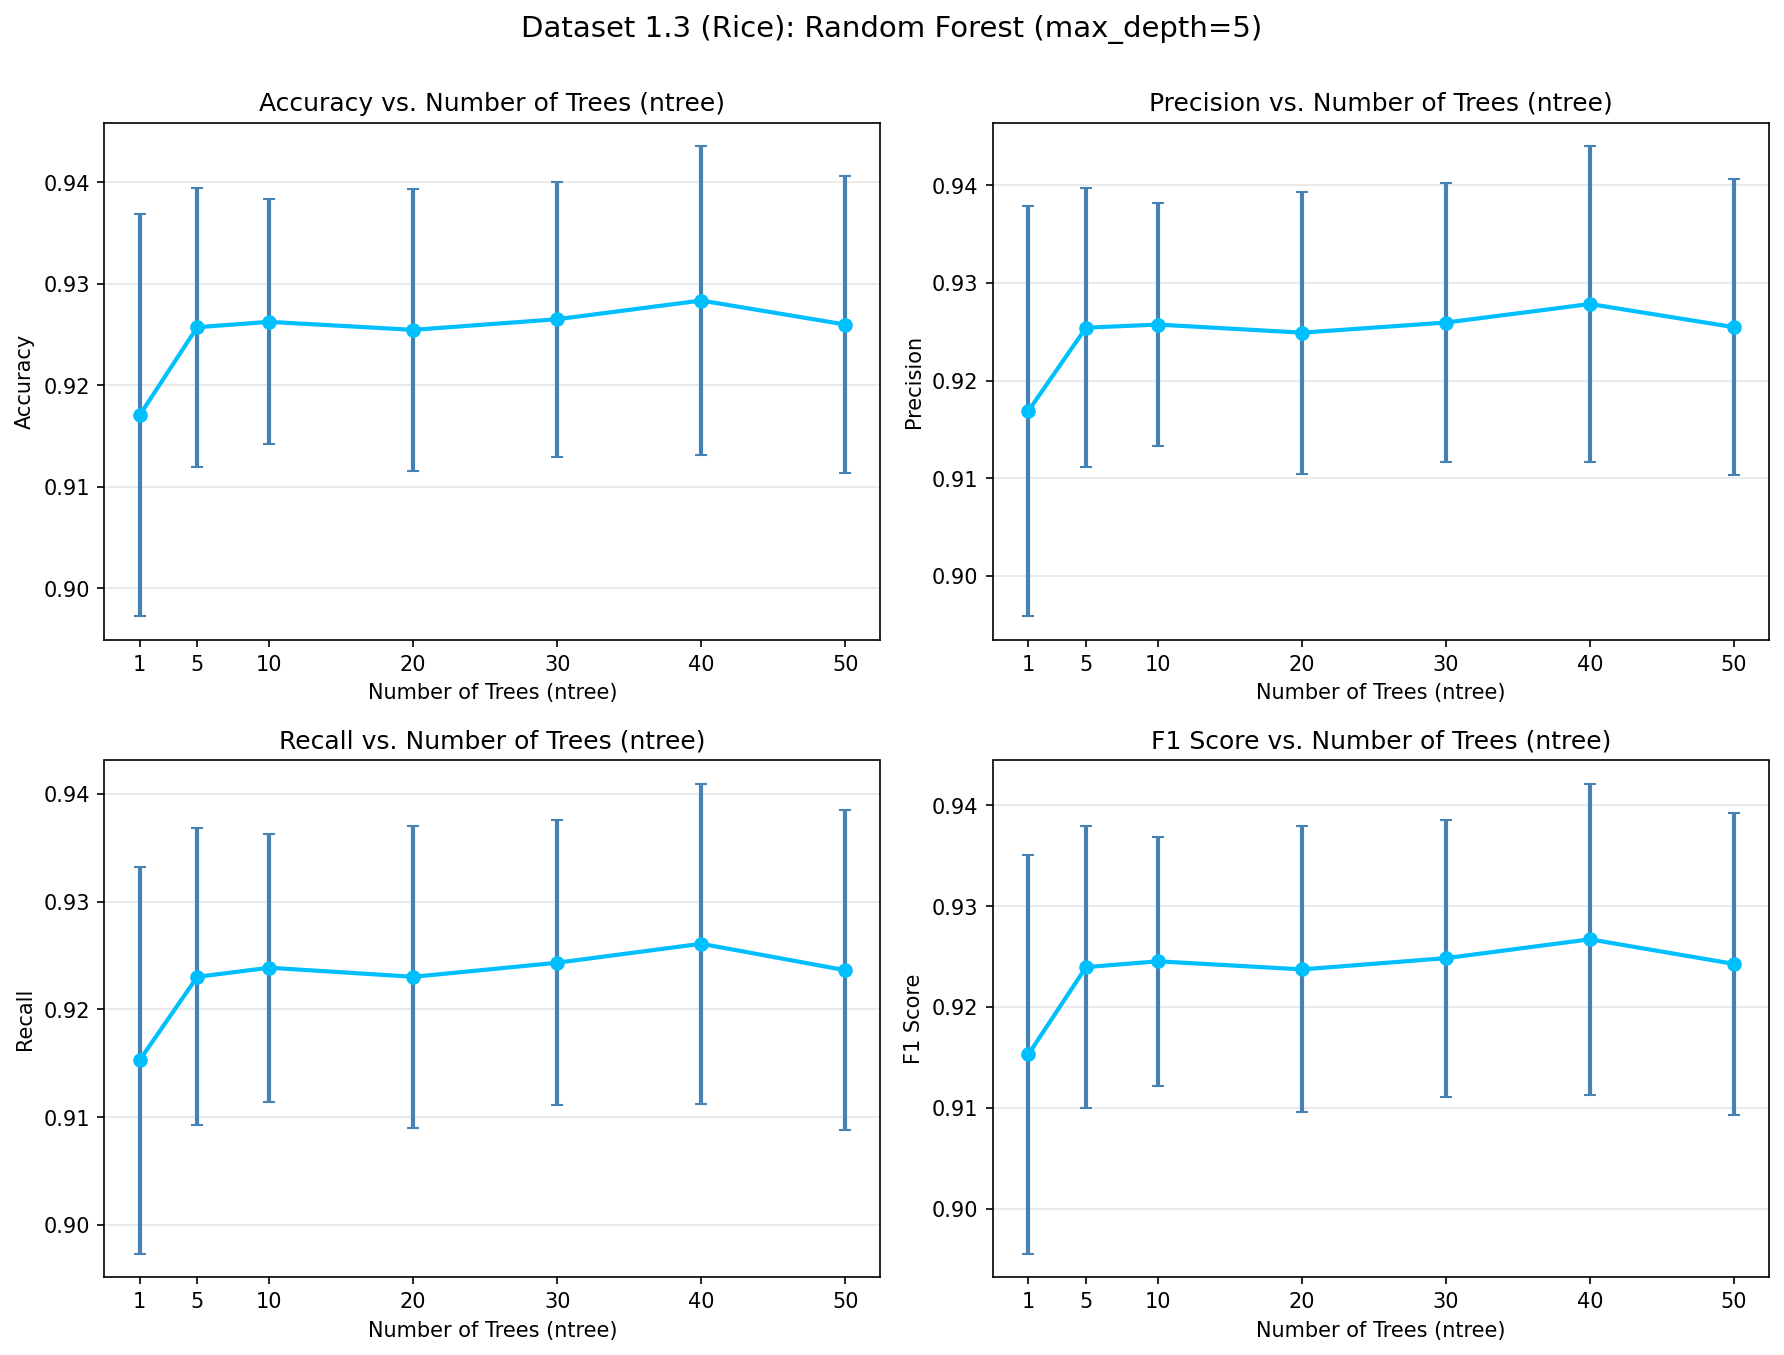
\includegraphics[width=0.8\linewidth]{figures/rice_rf_metrics.png}
        \caption{ Random Forest Performance over Rice Varieties.}
        \label{}
    \end{minipage}

    \begin{minipage}{\linewidth}
        \captionsetup{type=figure}
        \centering
        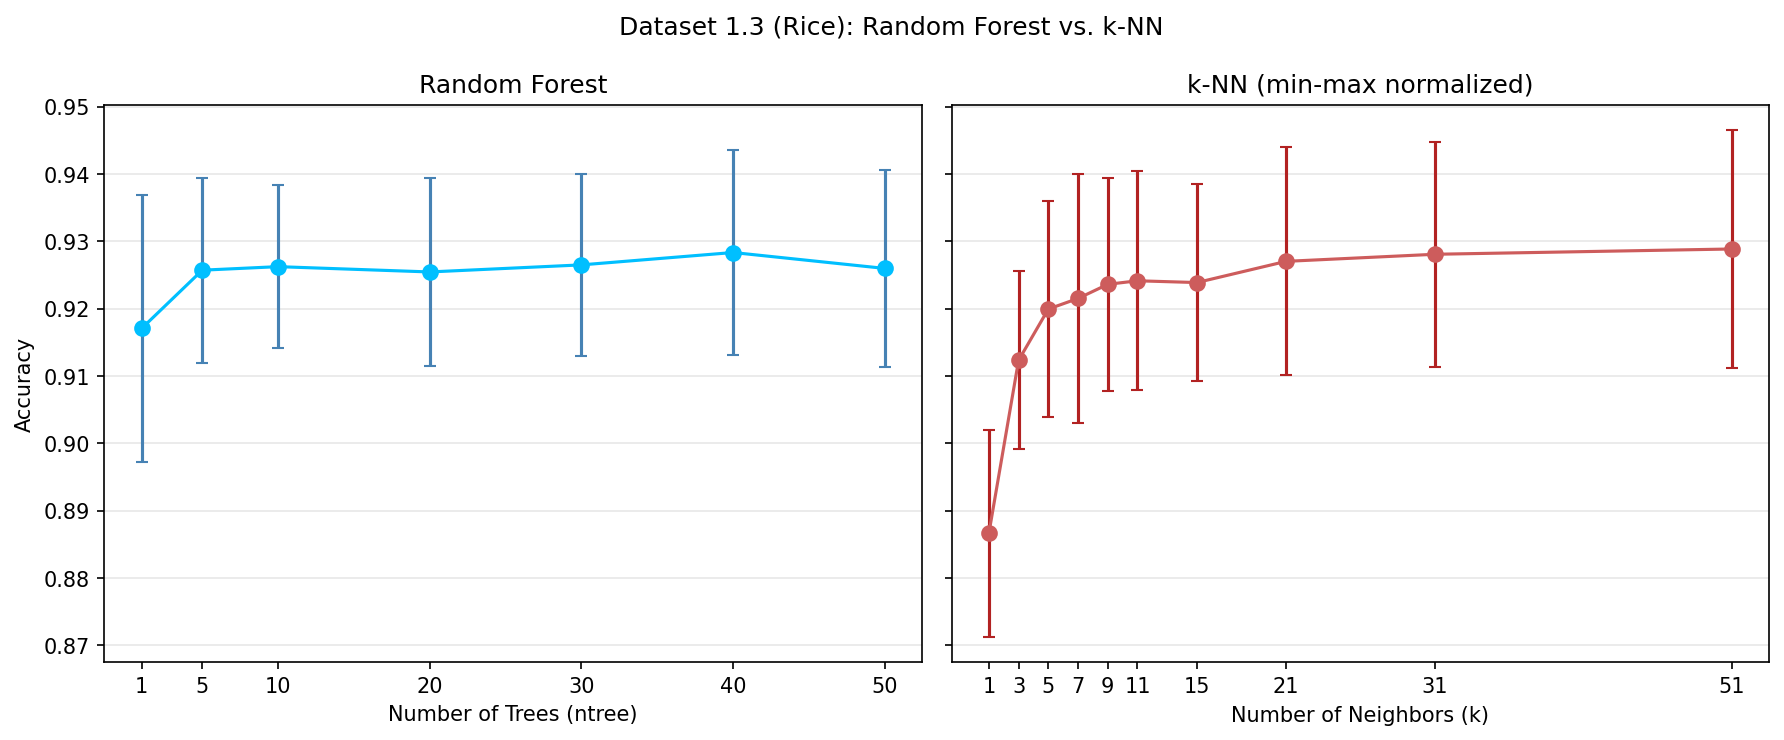
\includegraphics[width=0.8\linewidth]{figures/rice_comparison_rf_vs_knn.png}
        \caption{ Comparison of k-NN and RF over Rice Varieties.}
        \label{}
    \end{minipage}

\vspace{0.5cm}

\noindent {\Large{\textbf{D.} \textbf{ The Credit Approval Dataset}}}
\vspace{1.5cm}

    \begin{minipage}{\linewidth}
        \captionsetup{type=figure}
        \centering
        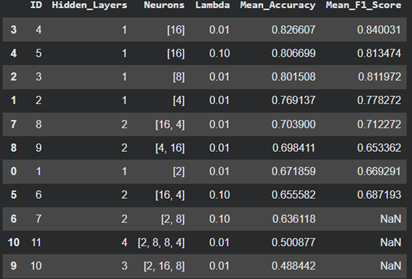
\includegraphics[width=0.7\linewidth]{figures/table_perf_credit.png}
        \caption{ Performance table using NN.}
        \label{}
    \end{minipage}

\vspace{0.5cm}

    \begin{minipage}{\linewidth}
        \captionsetup{type=figure}
        \centering
        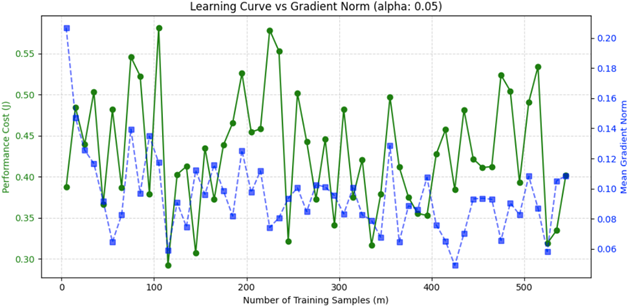
\includegraphics[width=0.9\linewidth]{figures/cradi_point4_poor_local.png}
        \caption{Learning curve vs. Gradient Norm in NN.}
        \label{}
    \end{minipage}

\vspace{0.5cm}

\noindent Table in the Figure 10 was obtained by modifying the hyperparameters: 1. the neural network architecture, and 2. the parameter that regulates J (lambda), all at a learning rate of alpha = 0.5. This is shown in Figure 10. These regulations are applied to the training folds using cross-validation. It can be noted that the credit approval predictor does not require an architecture exceeding one hidden layer; on the contrary, configuring it with two layers increases the failure rate—meaning, misclassified bad credit payers. This is supported by the F1-Score metric, which decreases in ID 9 (2 layers) compared to ID 4 (one layer). It can also be observed in the table that accuracy decreases as a function of a more complex neural network architecture.

Regarding poor local minimum, Figure 11 displays a graph with a learning rate of 0.05 for the best-performing architecture, which was [1 16 1] with a regularization parameter of 0.01. We can see that by reducing the learning rate from 0.5 to 0.05, the neurons become 'lazy' and enter a poor local minimum, as shown in the green plot. This graph demonstrates that J is not monotonically decreasing, exhibiting high variance and non-convergence. This induces a large error that is not corrected over time.
\vspace{1.5cm}

    \begin{minipage}{\linewidth}
        \captionsetup{type=figure}
        \centering
        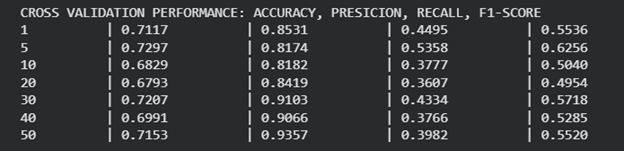
\includegraphics[width=0.8\linewidth]{figures/Table_perf_RT.png}
        \caption{ Performance table using Random Tree.}
        \label{}
    \end{minipage}

\vspace{0.5cm}

    \begin{minipage}{\linewidth}
        \captionsetup{type=figure}
        \centering
        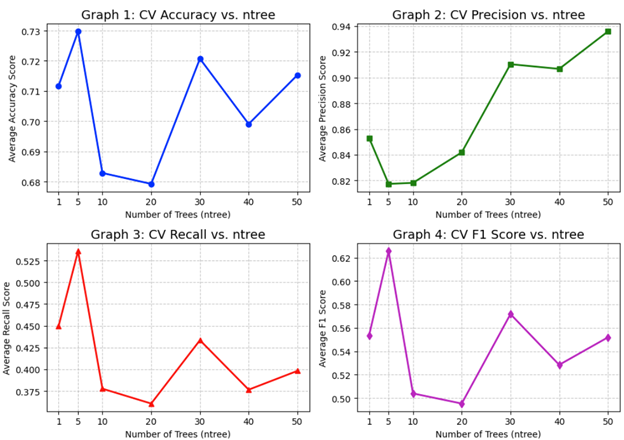
\includegraphics[width=0.8\linewidth]{figures/Table_perf_RT_2.png}
        \caption{ Performance table using Random Tree.}
        \label{}
    \end{minipage}

\vspace{0.5cm}

\noindent At first glance, it could be inferred that the optimal model is achieved with ntree=5 (where local peaks in accuracy and recall are observed). However, when analyzing the trend of the precision metric, a sustained improvement is observed starting from ntree=20.
Therefore, it is determined that the parameter offering the most robust model is ntree=30. At this point, the system achieves a superior balance between F1-Score and Accuracy, stabilizing the overall performance and reaching the second-highest precision value in the entire experiment without drastically sacrificing the other metrics.
Once the optimal model is selected, it is evaluated against the entire dataset to analyze its evolution across the performance metrics. This is illustrated in Figure 16. It is evident that the stability point for the metrics is reached at ntree=30, reinforcing the intuition regarding the robustness of the credit risk prediction model previously mentioned.

\vspace{0.5cm}
% ------------------------------------------
\noindent {\LARGE{\textbf{3. Analysis of the Best Hyperparameter}}} \
\vspace{0.5cm}


\noindent {\Large{\textbf{A.} \textbf{The Hand-Written Digits Recognition Dataset}}}\\
\vspace{0.5cm}

\noindent \textbf{RF:} number of trees $\mathit{ntree} \in \{1, 5, 10, 20, 30, 40, 50\}$ at fixed stopping criteria (\texttt{max\_depth=10}, \texttt{min\_size=2}, \texttt{min\_gain=0}). \textbf{k-NN:} number of neighbors $k \in \{1, 3, 5, 7, 9, 11, 15, 21, 31, 51\}$, evaluated both with min-max normalization (fit on train, applied to test) and on raw features.
\vspace{0.5cm}

\noindent For the Hand-written Digits dataset, the best tested setting of Random Forest was $\mathit{ntree}=50$, with an accuracy of $0.9739$ and F1 of $0.9738$. The results did point to the possibility that a larger $\mathit{ntree}$ might still provide better results. The k-NN approach however gave stronger results overall at both $k=3$ and $k=5$, with an accuracy of $0.9883$ and F1 of $0.9880$. The k-NN with $k=3$ would be the better setting to use on the Digits dataset.
\vspace{0.5cm}

\begin{minipage}{\linewidth}
    \captionsetup{type=figure}
    \centering
        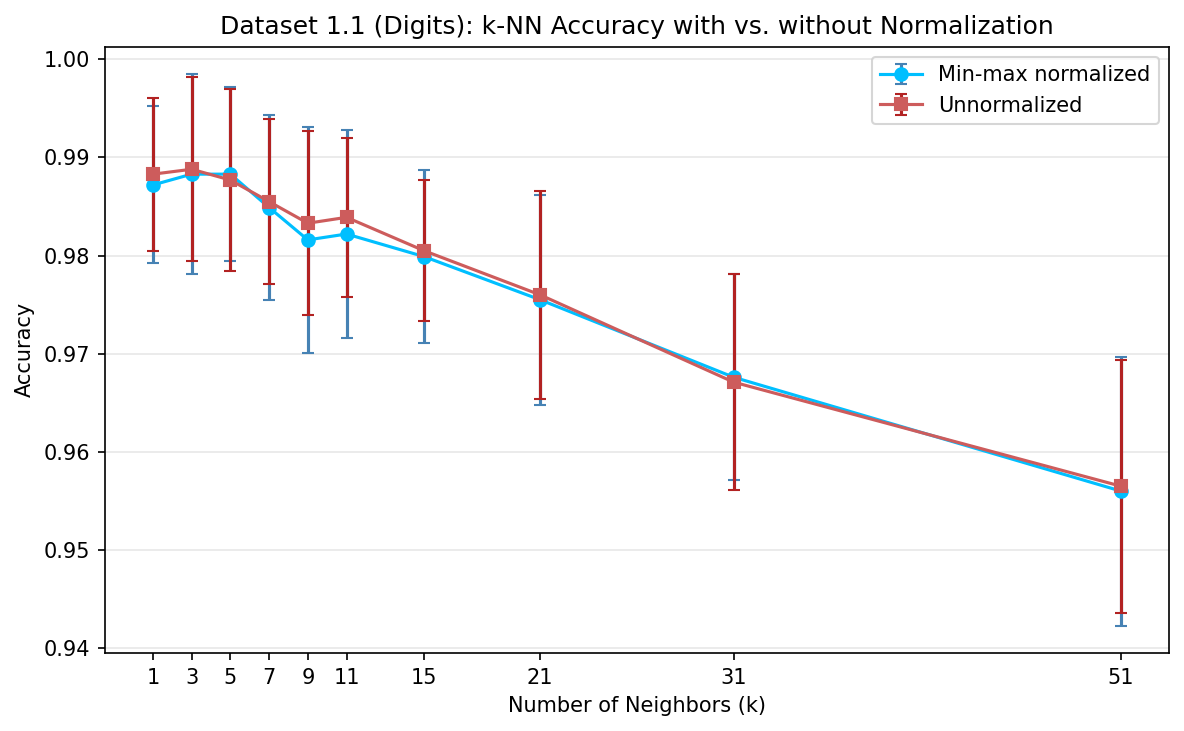
\includegraphics[width=0.8\linewidth]{figures/digits_knn_normalization_comparison.png}
        \caption{Normalization Comparison (Digits).}
        \label{fig:digits-knn-norm}
    \end{minipage}

\vspace{0.5cm}

\noindent On Digits, Random Forest keeps improving steadily out to $\mathit{ntree}=50$ and would likely continue to climb with more trees, while k-NN peaks early at $k=3$ to $5$ and then degrades as $k$ grows. Normalization is essentially a no-op here: the raw and min-max normalized k-NN curves overlap within noise, which is expected since every pixel is already on a uniform $0$ to $16$ scale and the L2 distance is therefore not dominated by any single feature.
\vspace{0.5cm}

\noindent To summarize for Digits, this is a 10-class problem with a uniform feature scale where k-NN ($k=3$) wins outright over Random Forest at the tested $\mathit{ntree}$ range, and normalization does not matter.
\vspace{0.5cm}

\noindent {\Large{\textbf{B.} \textbf{ The Oxford Parkinson’s Disease Detection Dataset}}}\\

\textbf{Neural Networks:}

\begin{figure}[H]
\centering
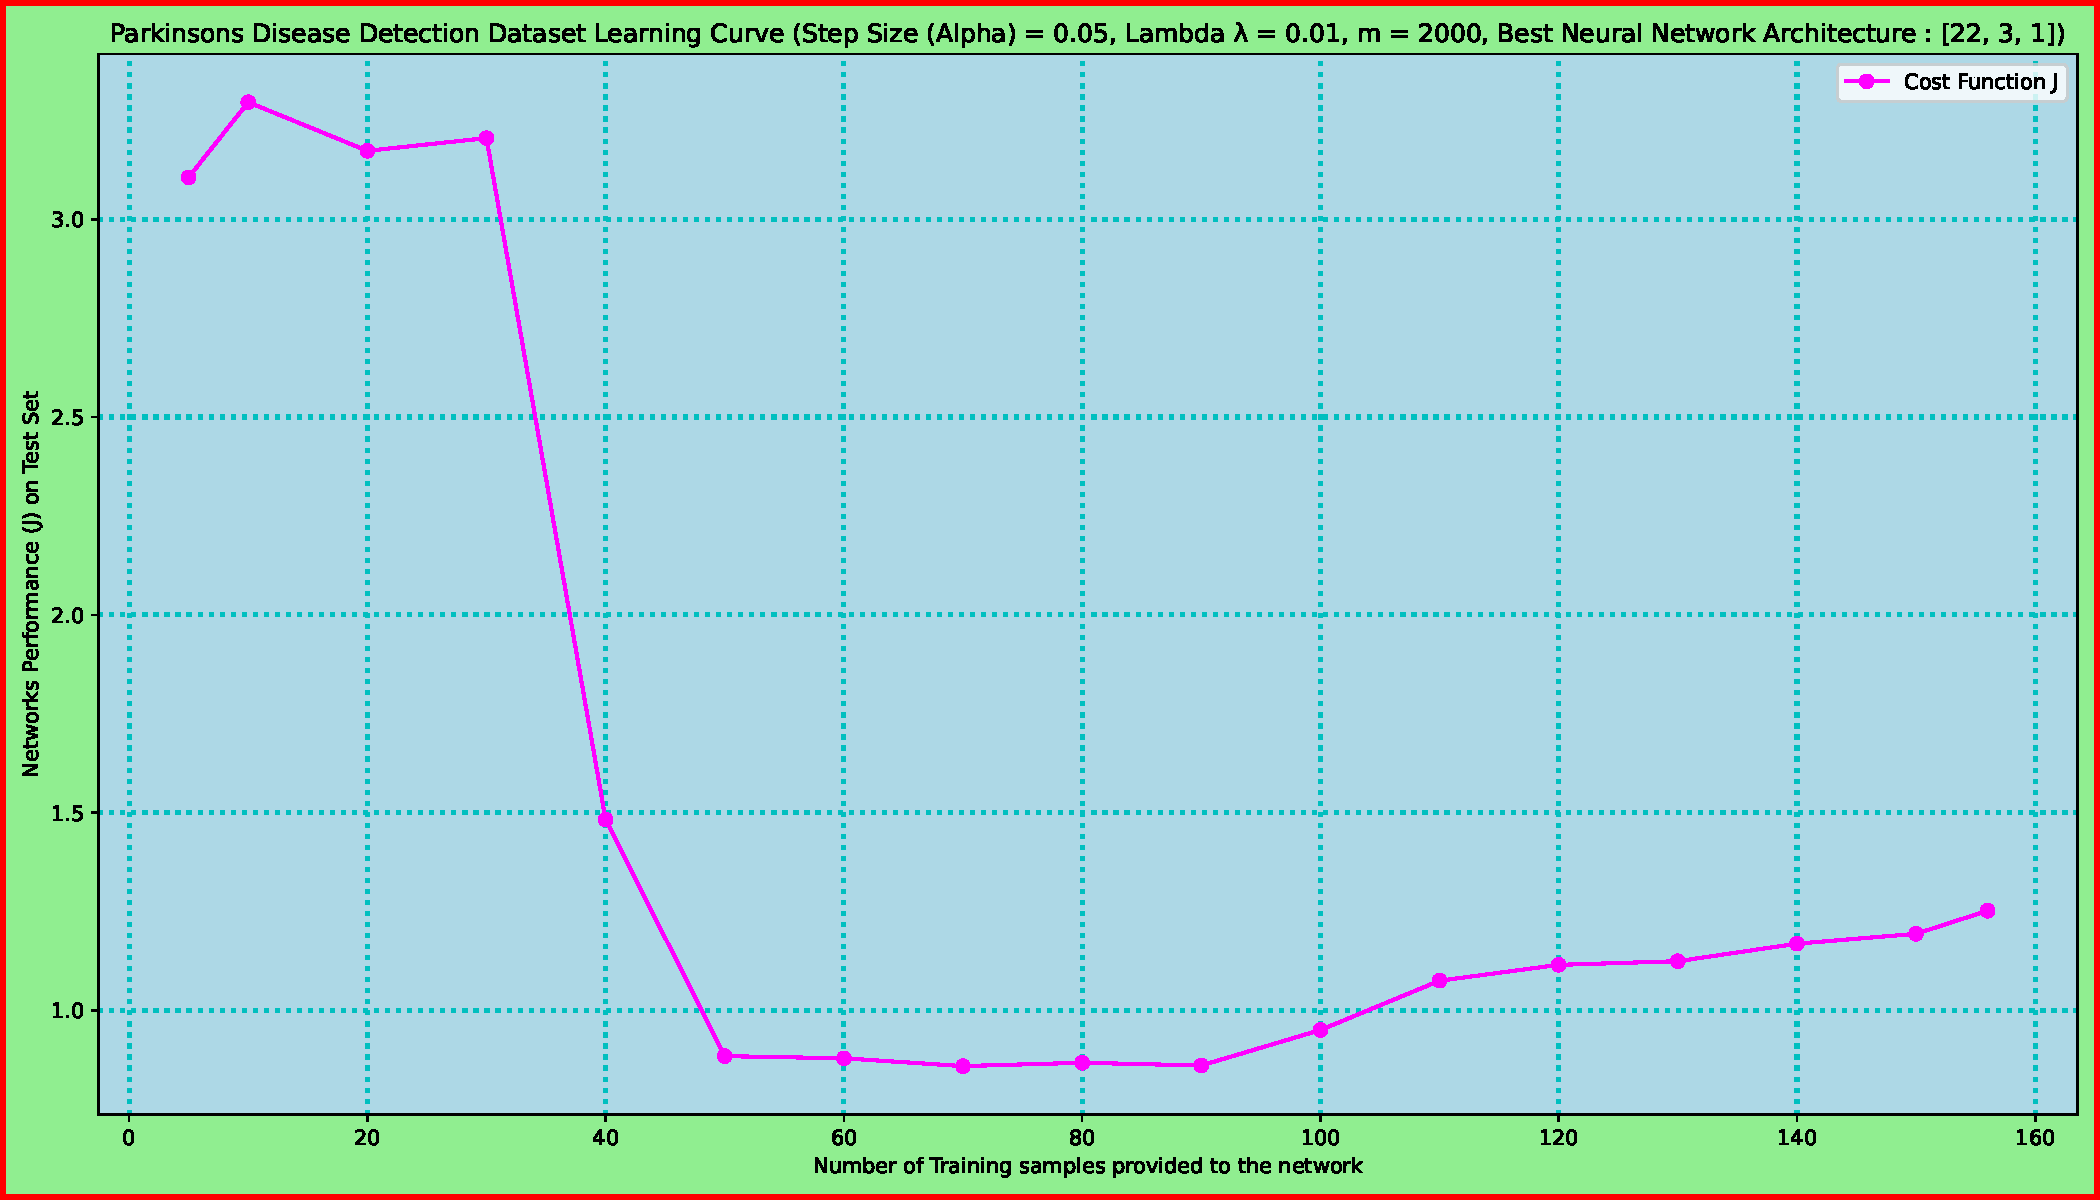
\includegraphics[width=0.8\textwidth]{figures/Parkinsons_Disease_Detection_Dataset_Learning_curve.pdf}
\caption{Learning curve for Neural Network on Parkinson’s Disease Detection Dataset}
\label{fig:learning_curve}
\end{figure}

\begin{enumerate}
    \item The step size $\alpha$ used for training this best neural network architecture is 0.05.

    \item The best neural network architecture used for the learning curve is [22, 3, 1].

    \item The regularization parameter $\lambda$ used for the learning curve is 0.01.

    \item The stopping criteria iteration is $m = 2000$.

    \item The Cost Function $J$ is initially high for training instances 5 to 30. This is because the network has few little training instances to learn meaningful pattern.

    \item The Cost Function $J$ decreases rapidly as the number of training size increases from 30 to 50. This indicates that the neural network model performance improves as the number of training data provided increases. The neural network rapidly learns the underlying patterns in the Parkinson's Disease Detection dataset.

    \item Beyond 50 training instances, the cost function $J$ stabilizes with minor fluctuations for higher training instances beyond 100. This indicates the model has generalized well and learning diminishes with additional training instances.

    \item The stabilization of the cost function for larger training sizes indicates that the model generalizes well with more training instances.

\end{enumerate}


\textbf{K-Nearest Neighbor:}

\begin{figure}[H]
\centering
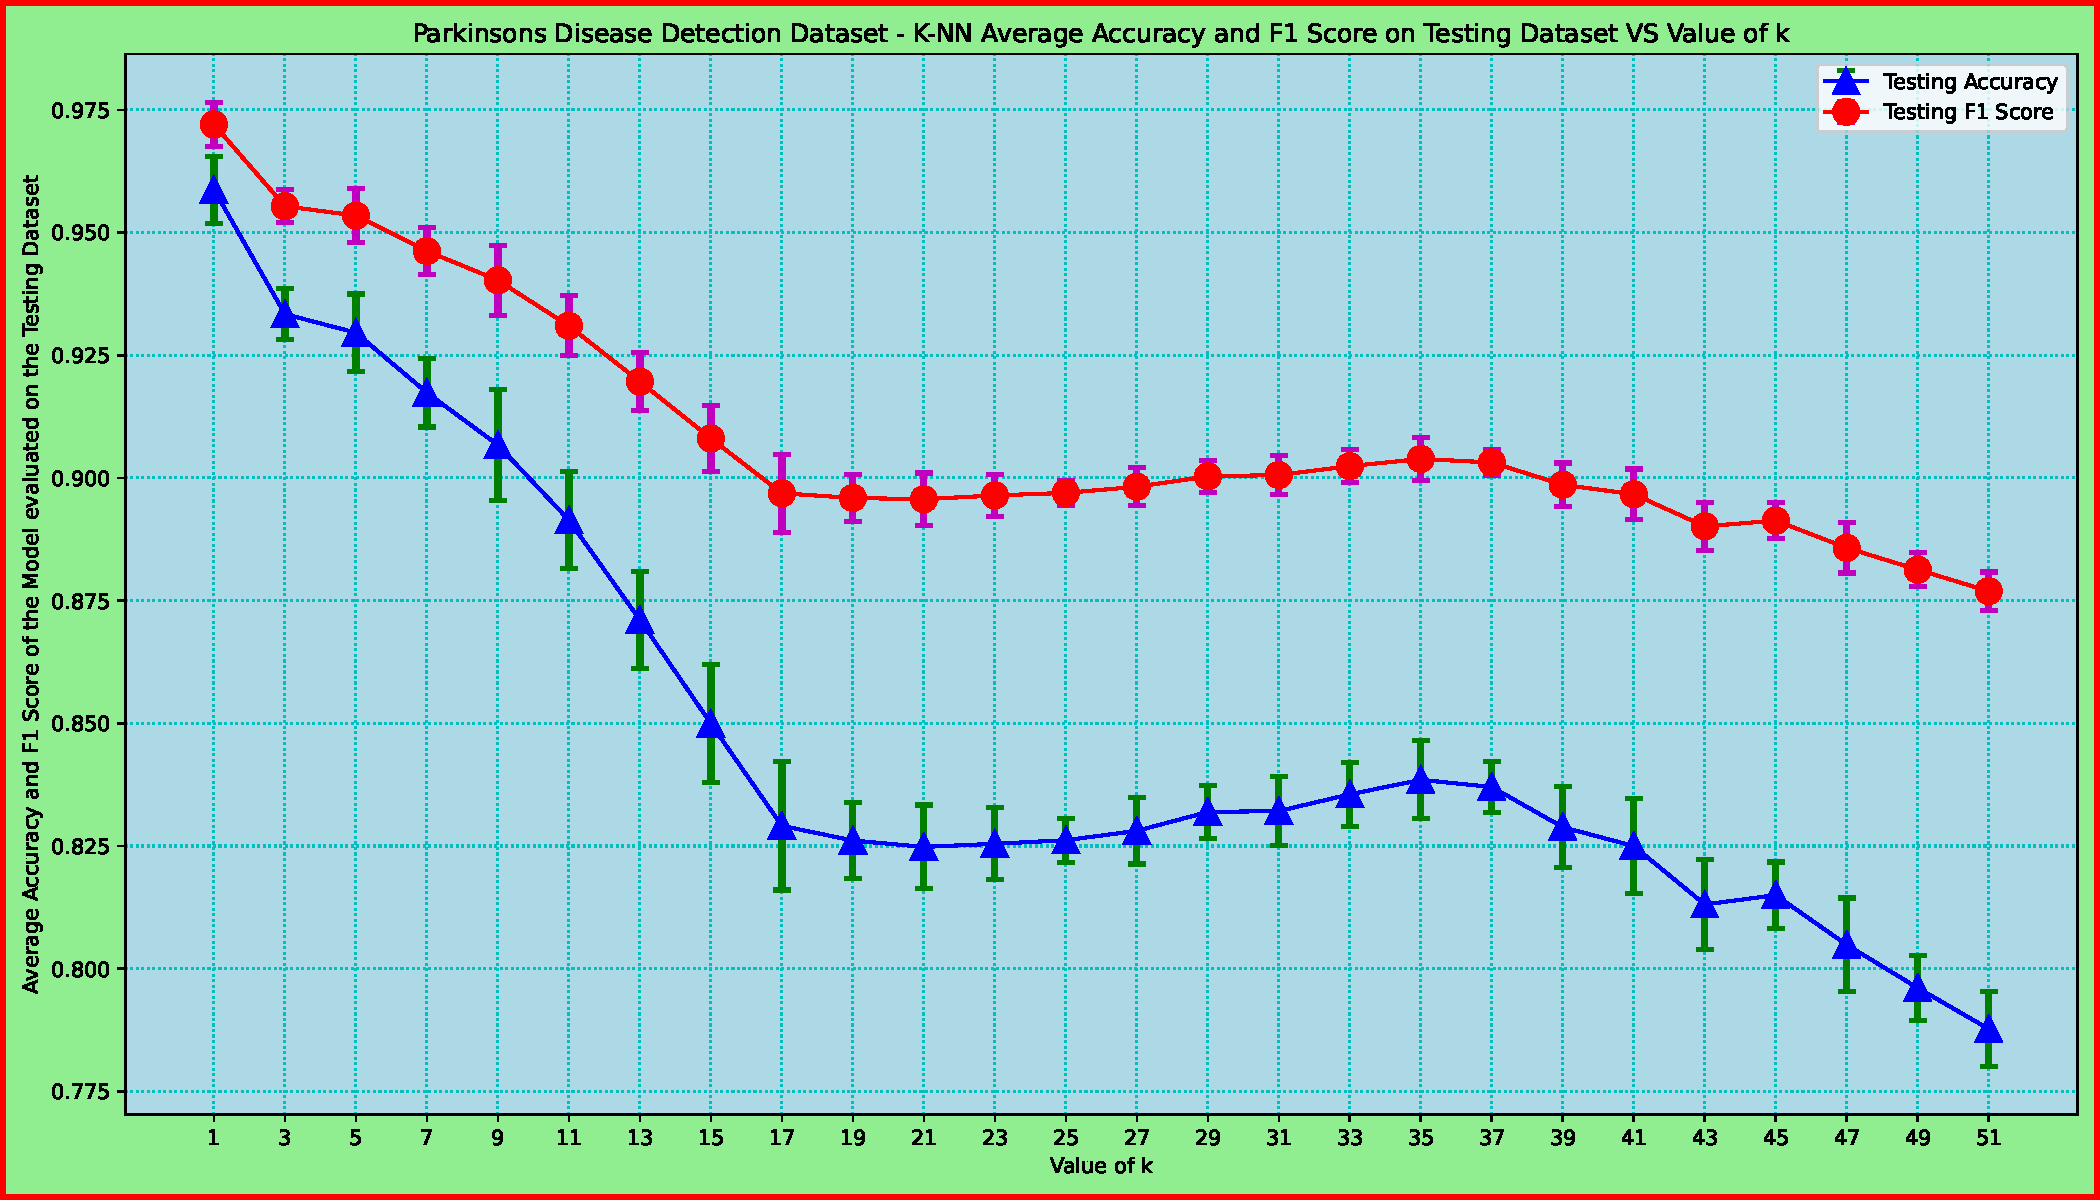
\includegraphics[width=0.8\textwidth]{figures/Parkinsons_kNN_Testing_Performance_vs_k.pdf}
\caption{K-Nearest Neighbor : Accuracy and F1-Score of the Testing Set for Parkinson’s Disease Detection Dataset}
\label{fig:learning_curve}
\end{figure}

\begin{enumerate}

    \item For $K = 3$ and $K = 5$, the K-NN model achieves peak performance with better generalization compared to $K = 1$. These values of $K$ effectively capture the underlying patterns correctly and makes higher accuracy and F1-score predictions in the Parkinson's Disease Detection dataset.

    \item For $K = 3$ and $K = 5$, the error bars are relatively small, which proves the models higher accuracy and F1-Score predictions are more robust across different data shuffles.

    \item For $K = 7$ to $K = 17$, the accuracy and F1-Score decreases significantly. From $K = 19$ to $K = 37$ the accuracy and F1 Score metrics flatten. Finally from $K = 39$ to $K = 51$, the accuracy and F1-score drops. This overall pattern indicates underfitting as $k$ value increases

    \item As $k$ increases, the number of instances considered for comparison from the training set increases, which drives both accuracy and F1-score down towards the majority class of the training dataset.

    \item For $k = 51$, the accuracy and F1-score of the k-NN model fall to their lowest points (Accuracy: 0.787721, F1-score: 0.876934), because the model becomes biased towards the majority class rather than predicting based on the underlying patterns in the data.

    \item For example, since the Parkinsons Disease Detection dataset has a majority of patients diagnosed with Parkinson's disease (class 1 = 75.4\%), with $k = 51$, the model will be more biased towards predicting that a person has Parkinson's disease regardless of their actual voice measurements of the patient. This is a classic sign of underfitting.

    \item For $K$ = 7 to 51, the error bars variance increases slightly which indicates the model has higher variability for higher $K$ values

    \item For $K = 1$, the model achieves highest test accuracy (0.958731) and F1-Score (0.972024). The model is overfitting to training data. If one of the neighbors is incorrect, it results in incorrect prediction. The model is highly sensitive to outliers and noise.

\end{enumerate}

\noindent {\Large{\textbf{C.} \textbf{ The Rice Grains Dataset}}}\\

\noindent \textbf{RF:} number of trees $\mathit{ntree} \in \{1, 5, 10, 20, 30, 40, 50\}$ at fixed stopping criteria (\texttt{max\_depth=5}, \texttt{min\_size=2}, \texttt{min\_gain=0}). \textbf{k-NN:} number of neighbors $k \in \{1, 3, 5, 7, 9, 11, 15, 21, 31, 51\}$, evaluated both with min-max normalization (fit on train, applied to test) and on raw features.
\vspace{0.5cm}

\noindent For the Rice Varieties dataset, the best Random Forest setting ended up at $\mathit{ntree}=40$, for an accuracy of $0.9283$ and F1 of $0.9267$. The best k-NN setting was a normalized approach with $k=51$, but there was little variation past $k=21$ overall. The resulting best setting provided an accuracy of $0.9289$ and F1 of $0.9273$. Both best approaches were close enough to be considered the same result within a fraction of a percent.
\vspace{0.5cm}

\noindent The two datasets of Hand-written digits and Rice varieties behave very differently. On Rice, RF stops improving by $\mathit{ntree}=10$ and k-NN keeps improving upwards as $k$ grows. On Digits, RF keeps improving out to $\mathit{ntree}=50$ while k-NN peaks at $k=3$ to $5$ and gets worse from there. Normalization also matters in different ways. It adds about 4 points of accuracy to k-NN on Rice, but does essentially nothing on Digits, since every pixel is already on a $0$ to $16$ scale.
\vspace{0.5cm}

\noindent To summarize, Rice is a binary problem with mixed feature scales where RF and k-NN tie and normalization is essential for k-NN. Digits is a 10-class problem with a uniform scale where k-NN wins and normalization doesn't matter. Very different outcomes between the same two algorithms but comparing them across datasets.
\vspace{0.5cm}

    \begin{minipage}{\linewidth}
        \captionsetup{type=figure}
        \centering
        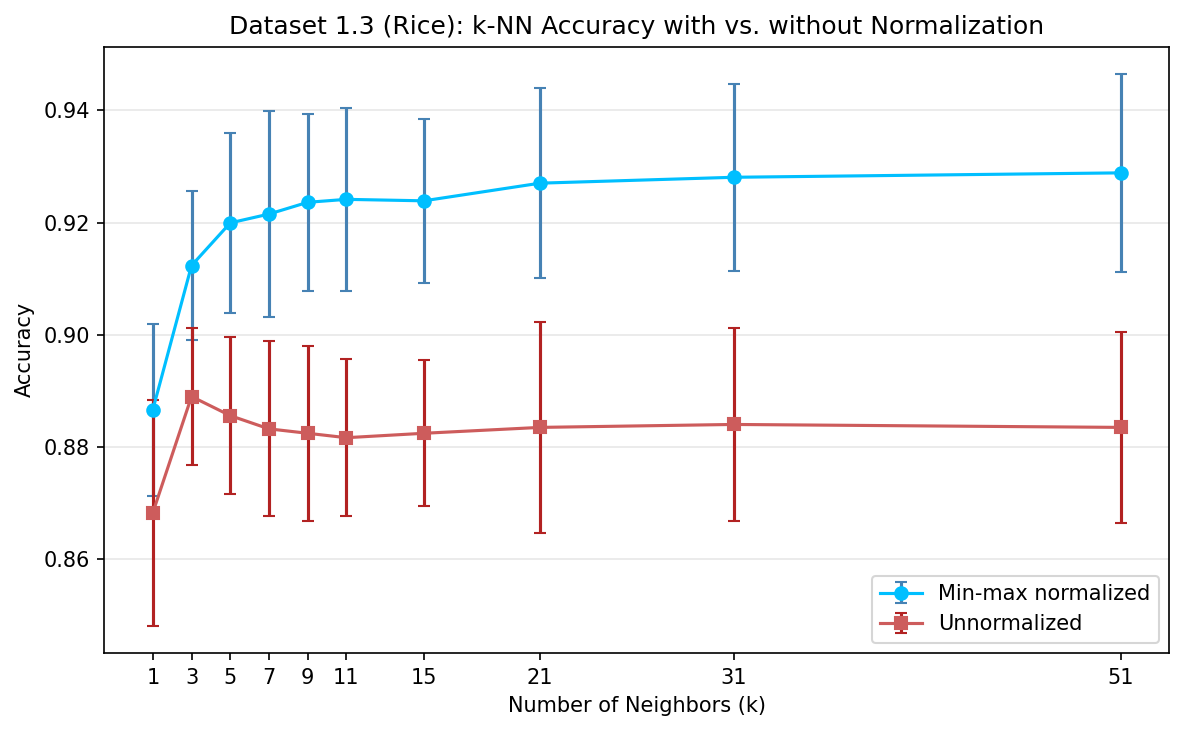
\includegraphics[width=0.8\linewidth]{figures/rice_knn_normalization_comparison.png}
        \caption{Normalization Comparison (Rice).}
        \label{fig:rice-knn-norm}
    \end{minipage}

\noindent {\Large{\textbf{D.} \textbf{The Credit Approval Dataset}}}

\vspace{0.5cm}

\noindent Based on the analysis in point 4. we can conclude that the optimal configuration is achieved with a [1 16 1] architecture, lambda = 0.01, and a learning rate of 0.5. The plot of J for these settings is shown in Figure 16. It satisfies the condition of being monotonic and effectively correcting the estimation error, with J stabilizing at a mean of 0.3.
This behavior confirms that the selected hyperparameters allow the model to generalize effectively without falling into the instability observed with lower learning rates. \\

\vspace{0.5cm}

\noindent Based on the analysis in point 4. it is evaluated against the entire dataset to analyze its evolution across the performance metrics. This is illustrated in Figure 17. Between ntree = 1 and ntree=10, the model is just beginning to learn. Stanting from ntree= 10 the model’s knowledge base is consolidated. It is evident that the stability point for the metrics is reached at tree=30, reinforcing the intuition regarding the robustness of the credit risk prediction model previously mentioned in point 4.


\vspace{1.5cm}

    \begin{minipage}{\linewidth}
        \captionsetup{type=figure}
        \centering
        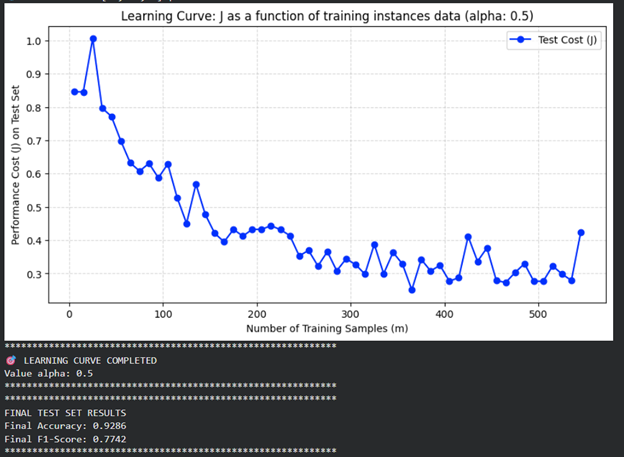
\includegraphics[width=0.7\linewidth]{figures/the_best_NN.png}
        \caption{ Analysis of the Best Hyperparameter in NN.}
        \label{}
    \end{minipage}
\vspace{1.5cm}

\begin{minipage}{\linewidth}
        \captionsetup{type=figure}
        \centering
        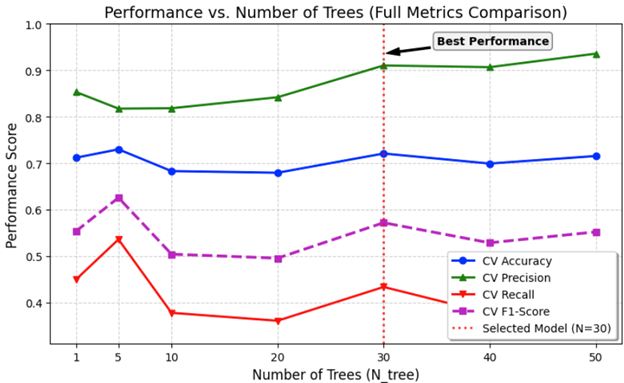
\includegraphics[width=0.8\linewidth]{figures/thebest_RT.png}
        \caption{ Analysis of the Best Hyperparameter in Random Tree.}
        \label{}
    \end{minipage}
% --------------------------------

\noindent {\LARGE{\textbf{4. Table Accuracy and F1-Score}}} \
\vspace{0.5cm}

\noindent {\Large{\textbf{A.} \textbf{The Hand-Written Digits Recognition Dataset}}}\\


\noindent {\Large{\textbf{B.} \textbf{ The Oxford Parkinson’s Disease Detection Dataset}}}\\

\noindent {\Large{\textbf{C.} \textbf{ The Rice Grains Dataset}}}\\


\noindent {\Large{\textbf{D.} \textbf{ The Credit Approval Dataset}}}
\vspace{1.5cm}



\begin{table}[H]
\centering
\resizebox{\textwidth}{!}{
\begin{tabular}{|l|c|c|c|c|c|c|c|c|}
\hline
 &
  \multicolumn{2}{c|}{\textbf{Hand-Written Digits}} &
  \multicolumn{2}{c|}{\textbf{Parkinson's Disease}} &
  \multicolumn{2}{c|}{\textbf{Rice Grains}} &
  \multicolumn{2}{c|}{\textbf{Credit Approval}} \\
\hline
\textbf{Algorithms} &
  \textbf{Accuracy} & \textbf{F1-Score} &
  \textbf{Accuracy} & \textbf{F1-Score} &
  \textbf{Accuracy} & \textbf{F1-Score} &
  \textbf{Accuracy} & \textbf{F1-Score} \\
\hline
K Nearest Neighbour & \cellcolor[HTML]{9B9B9B}\textbf{0.9883} & \cellcolor[HTML]{9B9B9B}\textbf{0.9883} & \cellcolor[HTML]{9B9B9B}\textbf{0.958731} & \cellcolor[HTML]{9B9B9B}\textbf{0.972024} & \cellcolor[HTML]{9B9B9B}\textbf{0.9289} & \cellcolor[HTML]{9B9B9B}\textbf{0.9273} & & \\
\hline
Random Forests & \textbf{0.9739} & \textbf{0.9738} & \textbf{0.928626} & \textbf{0.954540} & \textbf{0.9283} & \textbf{0.9267} & & \\
\hline
Decision Trees & & & & & & & & \\
\hline
Neural Networks & & & \textbf{0.866696} & \textbf{0.919369} & & & & \\
\hline
\end{tabular}}
\caption{Performance metrics comparison of algorithms on all four datasets}
\label{tab:final_results}
\end{table}


\section{Extra Credit}

{\Large \textbf{Extra Credit Question \#1}}
{\Large (10 Points)}

\vspace{0.3cm}

You may earn up to 10 extra points if you analyze all four datasets using an additional algorithm. In other words, you would be evaluating more than two algorithms on each of the datasets discussed in Section 1.

\bigskip

\textcolor{red}{\large{\textbf{I completed Extra Credit Question \#1 for The Oxford Parkinson’s Disease Detection Dataset, and the details of the results are presented below.}}}

\vspace{0.3cm}

\noindent {\Large{\textbf{ The Oxford Parkinson’s Disease Detection Dataset}}}\\

\vspace{0.3cm}

\noindent The Random Forest algorithm was selected as the third algorithm for the Oxford Parkinson's Disease Detection Dataset for the following reasons: Random Forest is one of the most widely used supervised machine learning algorithms in real-life applications. It often achieves state-of-the-art performance across a wide range of classification problems, making it a strong candidate for medical diagnosis tasks such as Parkinson's Disease Detection. Each tree in the Random Forest is trained on a different bootstrap dataset created by sampling with replacement from the original training dataset. This ensures each tree learns from a slightly different version.

\vspace{0.3cm}

A Random Forest classifier was trained and evaluated using the stratified cross-validation technique. The random forest model was trained with different values of the \textit{ntree} parameter. The performance metrics, including Accuracy, and F1-Score, along with their corresponding graphs and explanations, are discussed in the following sections.

\vspace{0.3cm}

The following stopping criteria were used while training and validating the Random Forest model: maximum depth = 10, minimum split size = 5, and information gain $\leq 0.01$.

Stratified cross-validation with $k = 10$ was used to evaluate random forest model performance.

\vspace{0.3cm}

\textbf{Accuracy, and F1-Score of the Random Forest for the Oxford Parkinson’s Disease Detection Dataset for each value of \textit{ntree}}


\begin{figure}[H]
    \centering
    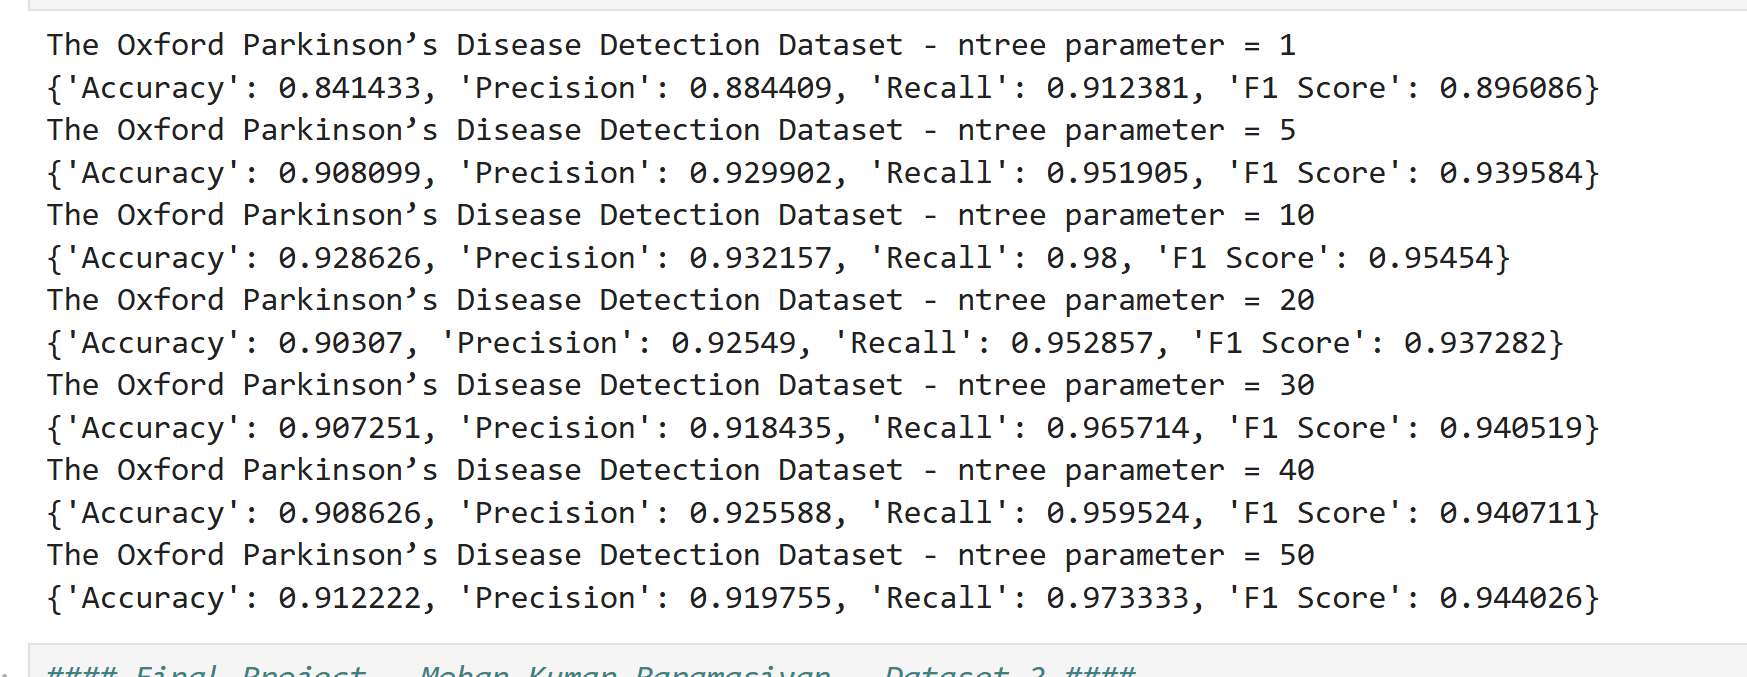
\includegraphics[width = 1.0\linewidth]{figures/image.png}
    \caption{Performance Metrics - Accuracy and F1-score for Parkinsons Disease Detection dataset for different values of \textit{ntree}}
    \label{fig:placeholder}
\end{figure}

\begin{table}[H]
\centering
\Large
\begin{tabular}{|c|c|c|}
\hline
\textbf{ntree} & \textbf{Accuracy} & \textbf{F1-Score} \\
\hline
1  & 0.841433 & 0.896086 \\
\hline
5  & 0.908099 & 0.939584 \\
\hline
\textbf{10} & \textbf{0.928626} & \textbf{0.954540} \\
\hline
20 & 0.903070 & 0.937282 \\
\hline
30 & 0.907251 & 0.940519 \\
\hline
40 & 0.908626 & 0.940711 \\
\hline
50 & 0.912222 & 0.944026 \\
\hline
\end{tabular}
\caption{Accuracy and F1-Score of the Random Forest Model for Different Values of \textit{ntree} on the Oxford Parkinson’s Disease Detection Dataset}
\label{tab:rf_parkinsons_accuracy_f1}
\end{table}

\large{\textbf{Best Hyperparameter Setting for the Random Forest Algorithm}} \\
\vspace{0.3cm}

\textbf{The best hyperparameter setting is $ntree = 10$ for the Random Forest algorithm, which resulted in the best performance with the highest accuracy of \textbf{0.928626} and the highest F1-Score of \textbf{0.954540} on the Oxford Parkinson's Disease Detection Dataset.}

\begin{table}[H]
\centering
\Large
\renewcommand{\arraystretch}{1.5}
\setlength{\tabcolsep}{20pt}
\begin{tabular}{|c|c|c|}
\hline
\textbf{ntree} & \textbf{Test Accuracy} & \textbf{Test F1-Score} \\
\hline
\textbf{10} & \textbf{0.928626} & \textbf{0.954540} \\
\hline
\end{tabular}
\caption{Best Hyperparameter Setting for the Random Forest Algorithm
on the Oxford Parkinson's Disease Detection Dataset}
\label{tab:rf_best_parkinsons}
\end{table}

\vspace{0.3cm}

\textbf{Accuracy of the random forest as a function of \textit{ntree} for the Oxford Parkinson’s Disease Detection Dataset}

\begin{figure}[H]
    \centering
    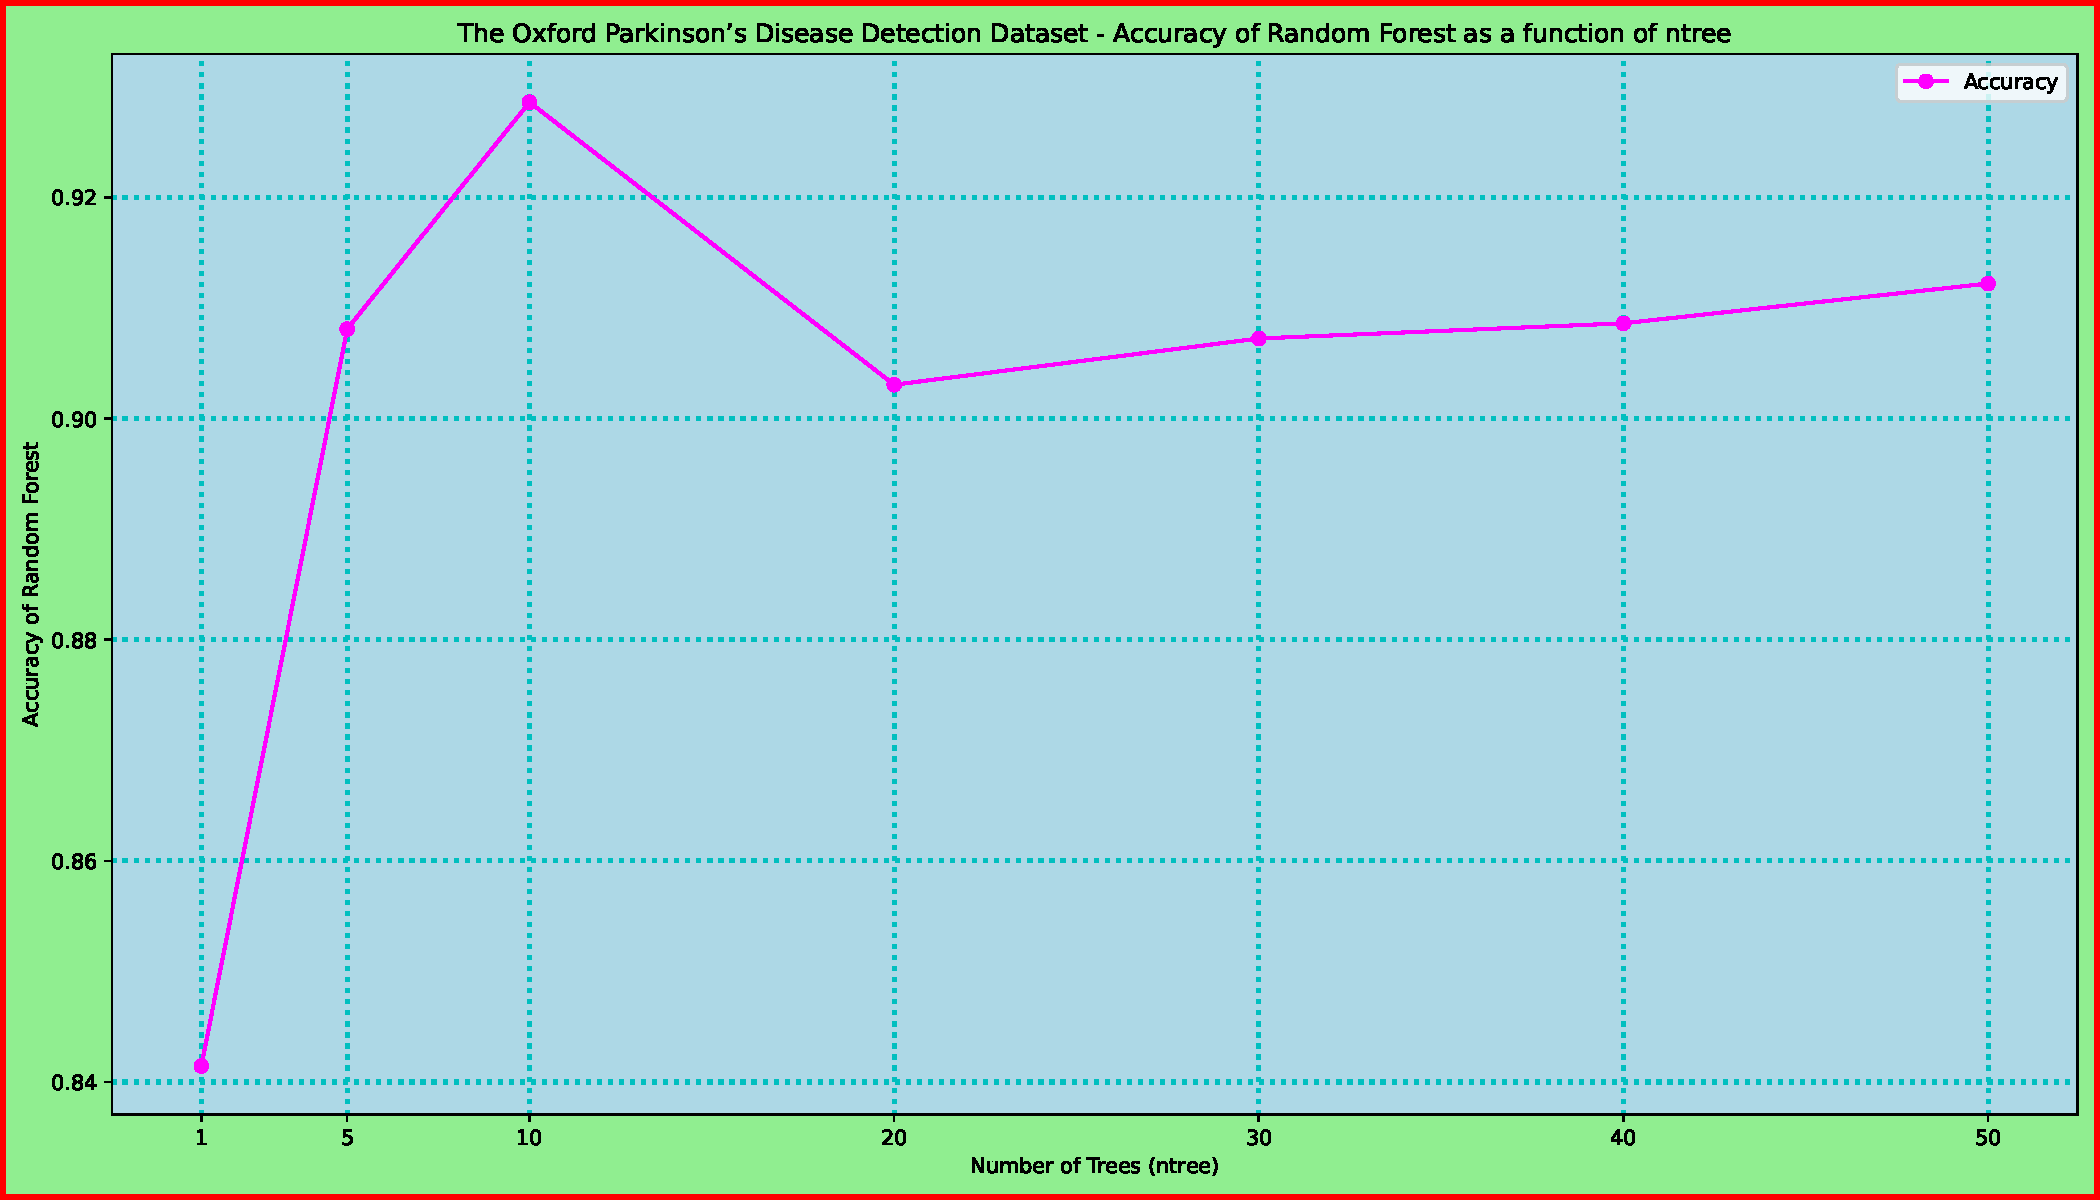
\includegraphics[width = 0.90\linewidth]{figures/Parkinsons_Accuracy.pdf}
    \caption{The Oxford Parkinson’s Disease Detection Dataset - Accuracy of the random forest as a
function of \textit{ntree}}
    \label{fig:placeholder}
\end{figure}


\textbf{F1-Score of the random forest as a function of \textit{ntree} for the Oxford Parkinson’s Disease Detection Dataset}

\begin{figure}[H]
    \centering
    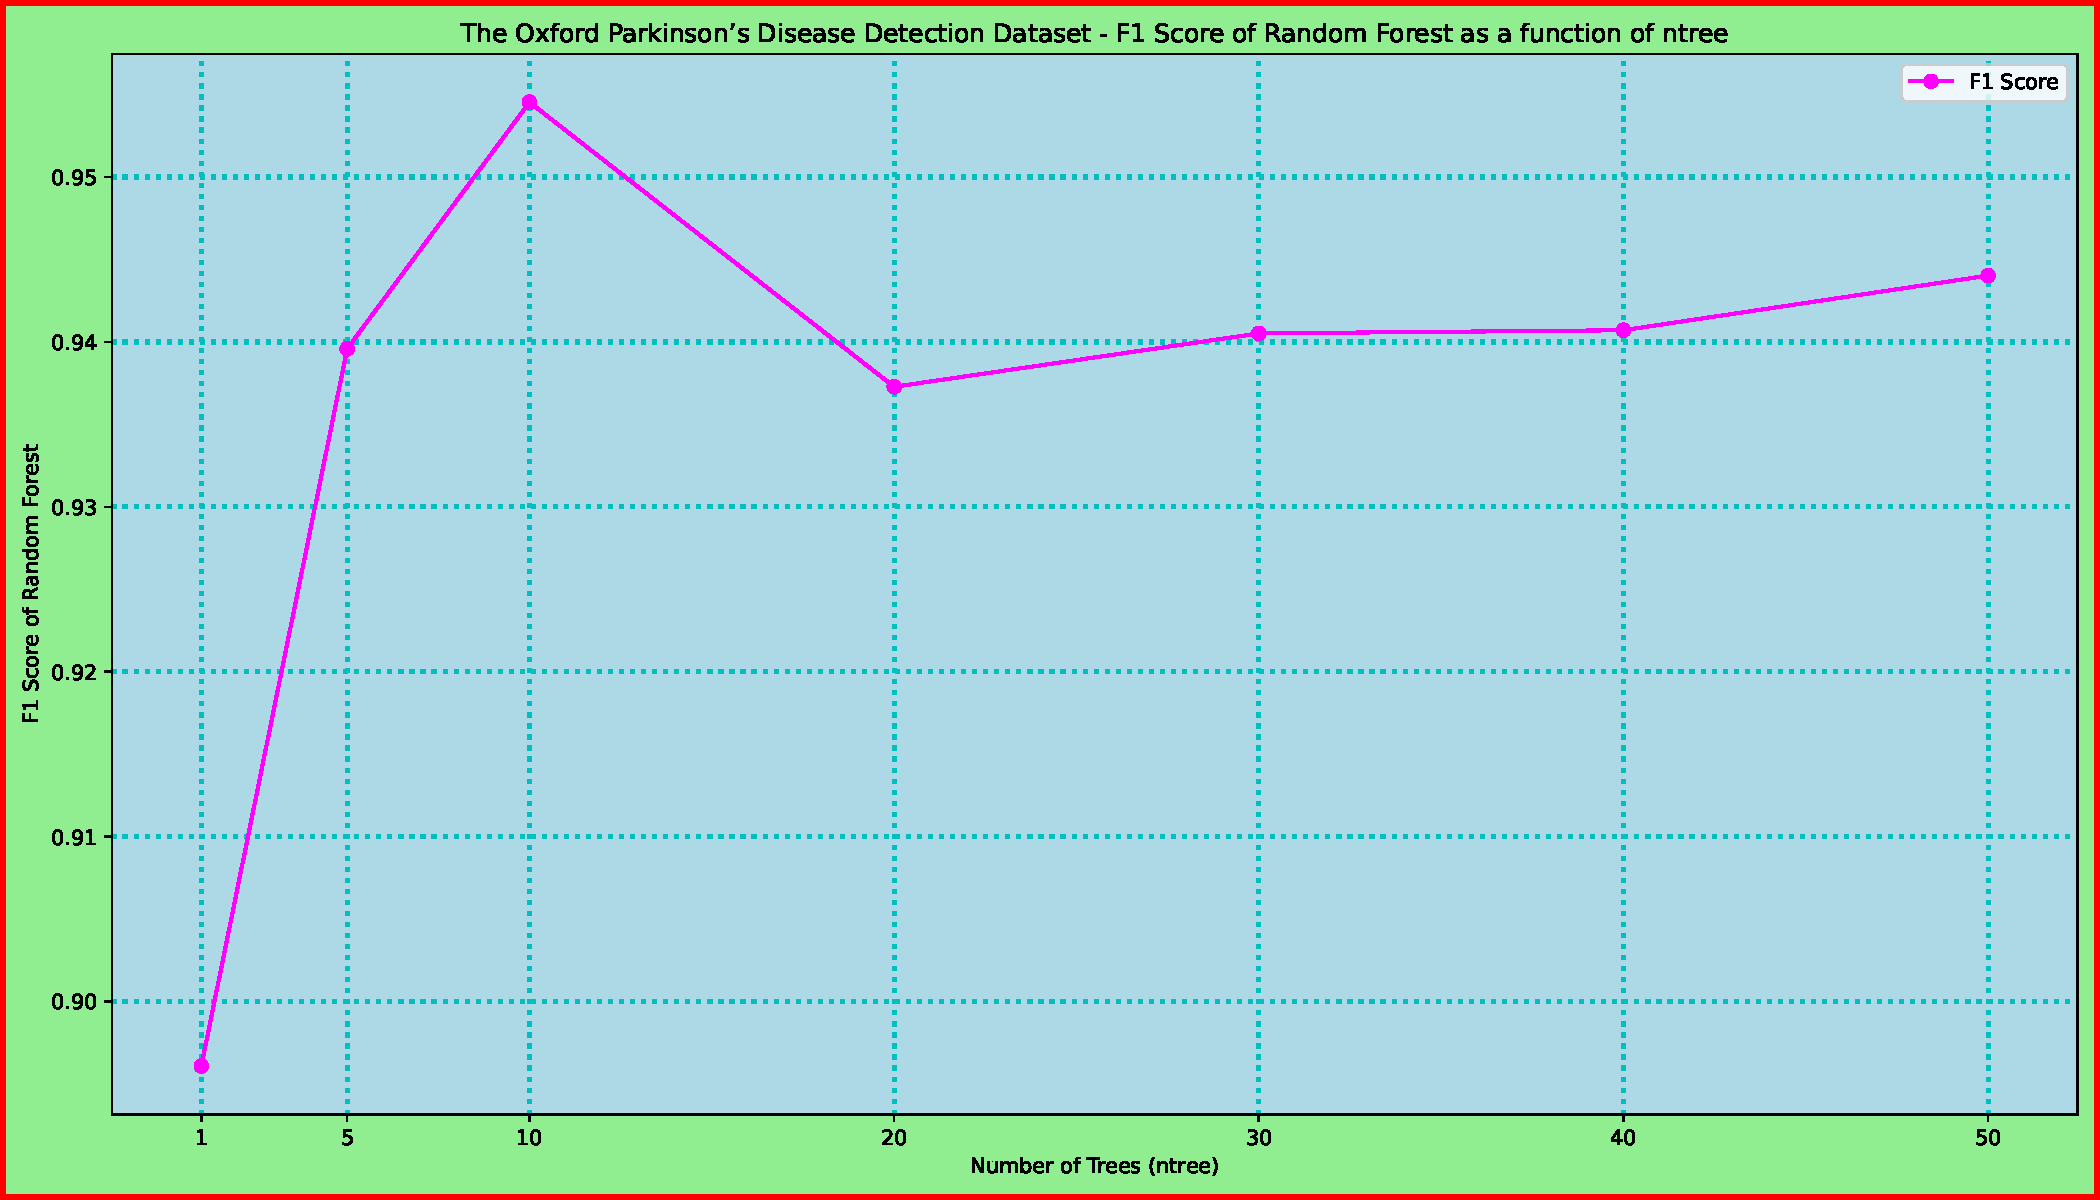
\includegraphics[width = 0.90\linewidth]{figures/Parkinsons_F1Score.pdf}
    \caption{The Oxford Parkinson’s Disease Detection Dataset - F1-Score of the random forest as a
function of \textit{ntree}}
    \label{fig:placeholder}
\end{figure}

\textbf{Accuracy:} If I were to deploy this classifier in a real-world application, I would choose $\textit{ntree} = 10$ for the Accuracy metric for the Oxford Parkinson’s Disease Detection Dataset. For $\textit{ntree} = 10$, the model achieves an Accuracy of 92.8626\%, which is the highest observed value. Beyond this point, the Accuracy decreases slightly and remains within the range of 90\% to 91\%.\\

Increasing the number of trees beyond $\textit{ntree} = 10$ does not provide any significant improvement in model performance, while the computational and training costs continue to increase. Therefore, selecting $\textit{ntree} = 10$ provides an effective balance between predictive performance and computational efficiency. The model is able to correctly classify approximately 93\% of the instances using this configuration.\\


\textbf{F1-Score:} If I were to deploy this classifier in a real-world application, I would choose $\textit{ntree} = 10$ for the F1-Score metric for the Oxford Parkinson’s Disease Detection Dataset. The F1-Score increases from $\textit{ntree} = 1$ to $\textit{ntree} = 10$ and reaches a maximum value of 95.454\%. Beyond this point, the F1-Score decreases slightly and remains within the range of 93.7\% to 94.5\%.\\

The difference in F1-Score between $\textit{ntree} = 10$ and higher values of $\textit{ntree}$ is minimal. Increasing the number of trees beyond $\textit{ntree} = 10$ does not provide any significant improvement in model performance, while the computational and training costs continue to increase. Therefore, selecting $\textit{ntree} = 10$ provides an effective balance between predictive performance and computational efficiency.



\end{document}
